% Options for packages loaded elsewhere
\PassOptionsToPackage{unicode}{hyperref}
\PassOptionsToPackage{hyphens}{url}
\PassOptionsToPackage{dvipsnames,svgnames,x11names}{xcolor}
%
\documentclass[
  letterpaper,
  DIV=11,
  numbers=noendperiod]{scrartcl}

\usepackage{amsmath,amssymb}
\usepackage{iftex}
\ifPDFTeX
  \usepackage[T1]{fontenc}
  \usepackage[utf8]{inputenc}
  \usepackage{textcomp} % provide euro and other symbols
\else % if luatex or xetex
  \usepackage{unicode-math}
  \defaultfontfeatures{Scale=MatchLowercase}
  \defaultfontfeatures[\rmfamily]{Ligatures=TeX,Scale=1}
\fi
\usepackage{lmodern}
\ifPDFTeX\else  
    % xetex/luatex font selection
\fi
% Use upquote if available, for straight quotes in verbatim environments
\IfFileExists{upquote.sty}{\usepackage{upquote}}{}
\IfFileExists{microtype.sty}{% use microtype if available
  \usepackage[]{microtype}
  \UseMicrotypeSet[protrusion]{basicmath} % disable protrusion for tt fonts
}{}
\makeatletter
\@ifundefined{KOMAClassName}{% if non-KOMA class
  \IfFileExists{parskip.sty}{%
    \usepackage{parskip}
  }{% else
    \setlength{\parindent}{0pt}
    \setlength{\parskip}{6pt plus 2pt minus 1pt}}
}{% if KOMA class
  \KOMAoptions{parskip=half}}
\makeatother
\usepackage{xcolor}
\setlength{\emergencystretch}{3em} % prevent overfull lines
\setcounter{secnumdepth}{-\maxdimen} % remove section numbering
% Make \paragraph and \subparagraph free-standing
\ifx\paragraph\undefined\else
  \let\oldparagraph\paragraph
  \renewcommand{\paragraph}[1]{\oldparagraph{#1}\mbox{}}
\fi
\ifx\subparagraph\undefined\else
  \let\oldsubparagraph\subparagraph
  \renewcommand{\subparagraph}[1]{\oldsubparagraph{#1}\mbox{}}
\fi

\usepackage{color}
\usepackage{fancyvrb}
\newcommand{\VerbBar}{|}
\newcommand{\VERB}{\Verb[commandchars=\\\{\}]}
\DefineVerbatimEnvironment{Highlighting}{Verbatim}{commandchars=\\\{\}}
% Add ',fontsize=\small' for more characters per line
\usepackage{framed}
\definecolor{shadecolor}{RGB}{241,243,245}
\newenvironment{Shaded}{\begin{snugshade}}{\end{snugshade}}
\newcommand{\AlertTok}[1]{\textcolor[rgb]{0.68,0.00,0.00}{#1}}
\newcommand{\AnnotationTok}[1]{\textcolor[rgb]{0.37,0.37,0.37}{#1}}
\newcommand{\AttributeTok}[1]{\textcolor[rgb]{0.40,0.45,0.13}{#1}}
\newcommand{\BaseNTok}[1]{\textcolor[rgb]{0.68,0.00,0.00}{#1}}
\newcommand{\BuiltInTok}[1]{\textcolor[rgb]{0.00,0.23,0.31}{#1}}
\newcommand{\CharTok}[1]{\textcolor[rgb]{0.13,0.47,0.30}{#1}}
\newcommand{\CommentTok}[1]{\textcolor[rgb]{0.37,0.37,0.37}{#1}}
\newcommand{\CommentVarTok}[1]{\textcolor[rgb]{0.37,0.37,0.37}{\textit{#1}}}
\newcommand{\ConstantTok}[1]{\textcolor[rgb]{0.56,0.35,0.01}{#1}}
\newcommand{\ControlFlowTok}[1]{\textcolor[rgb]{0.00,0.23,0.31}{#1}}
\newcommand{\DataTypeTok}[1]{\textcolor[rgb]{0.68,0.00,0.00}{#1}}
\newcommand{\DecValTok}[1]{\textcolor[rgb]{0.68,0.00,0.00}{#1}}
\newcommand{\DocumentationTok}[1]{\textcolor[rgb]{0.37,0.37,0.37}{\textit{#1}}}
\newcommand{\ErrorTok}[1]{\textcolor[rgb]{0.68,0.00,0.00}{#1}}
\newcommand{\ExtensionTok}[1]{\textcolor[rgb]{0.00,0.23,0.31}{#1}}
\newcommand{\FloatTok}[1]{\textcolor[rgb]{0.68,0.00,0.00}{#1}}
\newcommand{\FunctionTok}[1]{\textcolor[rgb]{0.28,0.35,0.67}{#1}}
\newcommand{\ImportTok}[1]{\textcolor[rgb]{0.00,0.46,0.62}{#1}}
\newcommand{\InformationTok}[1]{\textcolor[rgb]{0.37,0.37,0.37}{#1}}
\newcommand{\KeywordTok}[1]{\textcolor[rgb]{0.00,0.23,0.31}{#1}}
\newcommand{\NormalTok}[1]{\textcolor[rgb]{0.00,0.23,0.31}{#1}}
\newcommand{\OperatorTok}[1]{\textcolor[rgb]{0.37,0.37,0.37}{#1}}
\newcommand{\OtherTok}[1]{\textcolor[rgb]{0.00,0.23,0.31}{#1}}
\newcommand{\PreprocessorTok}[1]{\textcolor[rgb]{0.68,0.00,0.00}{#1}}
\newcommand{\RegionMarkerTok}[1]{\textcolor[rgb]{0.00,0.23,0.31}{#1}}
\newcommand{\SpecialCharTok}[1]{\textcolor[rgb]{0.37,0.37,0.37}{#1}}
\newcommand{\SpecialStringTok}[1]{\textcolor[rgb]{0.13,0.47,0.30}{#1}}
\newcommand{\StringTok}[1]{\textcolor[rgb]{0.13,0.47,0.30}{#1}}
\newcommand{\VariableTok}[1]{\textcolor[rgb]{0.07,0.07,0.07}{#1}}
\newcommand{\VerbatimStringTok}[1]{\textcolor[rgb]{0.13,0.47,0.30}{#1}}
\newcommand{\WarningTok}[1]{\textcolor[rgb]{0.37,0.37,0.37}{\textit{#1}}}

\providecommand{\tightlist}{%
  \setlength{\itemsep}{0pt}\setlength{\parskip}{0pt}}\usepackage{longtable,booktabs,array}
\usepackage{calc} % for calculating minipage widths
% Correct order of tables after \paragraph or \subparagraph
\usepackage{etoolbox}
\makeatletter
\patchcmd\longtable{\par}{\if@noskipsec\mbox{}\fi\par}{}{}
\makeatother
% Allow footnotes in longtable head/foot
\IfFileExists{footnotehyper.sty}{\usepackage{footnotehyper}}{\usepackage{footnote}}
\makesavenoteenv{longtable}
\usepackage{graphicx}
\makeatletter
\def\maxwidth{\ifdim\Gin@nat@width>\linewidth\linewidth\else\Gin@nat@width\fi}
\def\maxheight{\ifdim\Gin@nat@height>\textheight\textheight\else\Gin@nat@height\fi}
\makeatother
% Scale images if necessary, so that they will not overflow the page
% margins by default, and it is still possible to overwrite the defaults
% using explicit options in \includegraphics[width, height, ...]{}
\setkeys{Gin}{width=\maxwidth,height=\maxheight,keepaspectratio}
% Set default figure placement to htbp
\makeatletter
\def\fps@figure{htbp}
\makeatother

\KOMAoption{captions}{tableheading}
\makeatletter
\@ifpackageloaded{caption}{}{\usepackage{caption}}
\AtBeginDocument{%
\ifdefined\contentsname
  \renewcommand*\contentsname{Table of contents}
\else
  \newcommand\contentsname{Table of contents}
\fi
\ifdefined\listfigurename
  \renewcommand*\listfigurename{List of Figures}
\else
  \newcommand\listfigurename{List of Figures}
\fi
\ifdefined\listtablename
  \renewcommand*\listtablename{List of Tables}
\else
  \newcommand\listtablename{List of Tables}
\fi
\ifdefined\figurename
  \renewcommand*\figurename{Figure}
\else
  \newcommand\figurename{Figure}
\fi
\ifdefined\tablename
  \renewcommand*\tablename{Table}
\else
  \newcommand\tablename{Table}
\fi
}
\@ifpackageloaded{float}{}{\usepackage{float}}
\floatstyle{ruled}
\@ifundefined{c@chapter}{\newfloat{codelisting}{h}{lop}}{\newfloat{codelisting}{h}{lop}[chapter]}
\floatname{codelisting}{Listing}
\newcommand*\listoflistings{\listof{codelisting}{List of Listings}}
\makeatother
\makeatletter
\makeatother
\makeatletter
\@ifpackageloaded{caption}{}{\usepackage{caption}}
\@ifpackageloaded{subcaption}{}{\usepackage{subcaption}}
\makeatother
\ifLuaTeX
  \usepackage{selnolig}  % disable illegal ligatures
\fi
\usepackage{bookmark}

\IfFileExists{xurl.sty}{\usepackage{xurl}}{} % add URL line breaks if available
\urlstyle{same} % disable monospaced font for URLs
\hypersetup{
  pdftitle={Week 7: SVM models},
  colorlinks=true,
  linkcolor={blue},
  filecolor={Maroon},
  citecolor={Blue},
  urlcolor={Blue},
  pdfcreator={LaTeX via pandoc}}

\title{Week 7: SVM models}
\author{}
\date{}

\begin{document}
\maketitle

The following information is summarized from Géron (2019) book.

\begin{figure}[H]

{\centering 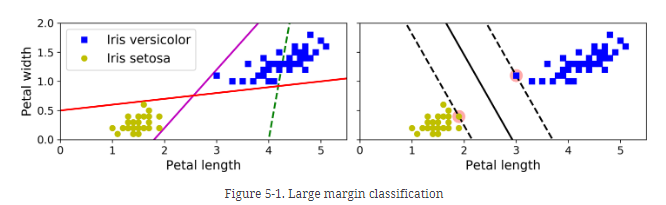
\includegraphics{1.png}

}

\caption{picture}

\end{figure}%

This picture demonstrate the decision boundaries. On the left, there are
3 decision boundaries, the green one doesn't amount to anything, the
purple and red one, although they separate the data quite nicely on the
training set, but won't generalize well on test set.

On the right, it is the SVM classier, the decision boundary separates 2
classes and stays away as far as possible from the closet training
instances. We called this \textbf{large margin classification}, where
the decision boundary is determined by the closest instances to the
decision boundary which is called \textbf{support vectors}.

\subsection{7.1 Soft Margin
Classification}\label{soft-margin-classification}

What we see in the above example is \textbf{hard margin classification}
where all instance must be on the right side. However, it only works if
the data is linearly separable, and sensitive to outliers. The picture
below will demonstrate that if we add one instance on of the wrong
class, the decision boundary will not be drawn, or drawn but not
generalize well.

\begin{figure}[H]

{\centering 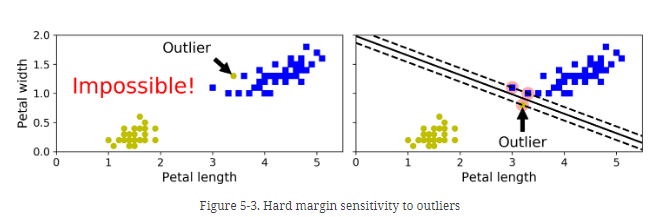
\includegraphics{2.png}

}

\caption{picture}

\end{figure}%

To avoid this, we need to use a more flexible model or \textbf{soft
margin classification} model, where it finds a good balance for the
decision boundary margin and avoid \emph{margin violations} (instances
in the middle of the margin or wrong side).

The hyperparameter \texttt{C} will control the trade-off between
maximizing the margin and minimizing the classification error. The
picture below shows the 2 case scenarios. On the left where \texttt{C}
is small, it might not fit the data well (margin violations), but
generalize the model by maximizing the margin between classes. On the
right where \texttt{C} is high, the model is less tolerant to
misclassified because of smaller margin, but this could lead to
overfitting.

\subsection{7.2 Nonlinear SVM
Classification}\label{nonlinear-svm-classification}

SVM has something called the \textbf{kernel trick}, where it computes
the dot product of the original data points \texttt{X} and the
transformed \texttt{X\textquotesingle{}} in a high dimensional space
without explicitly transforming the data into that space.

The transformed data depends on the \textbf{kernel functions}, and there
are a few popular ones like linear, polynomial, RBF and sigmoid.

\subsubsection{7.2.1 Polynomial Kernel}\label{polynomial-kernel}

It works similar to adding polynomial features without adding polynomial
features. The picture below will show SVM classifier with different
degree of polynomial.

\begin{Shaded}
\begin{Highlighting}[]
\ImportTok{from}\NormalTok{ sklearn.datasets }\ImportTok{import}\NormalTok{ make\_moons}
\ImportTok{from}\NormalTok{ sklearn.pipeline }\ImportTok{import}\NormalTok{ Pipeline}
\ImportTok{from}\NormalTok{ sklearn.preprocessing }\ImportTok{import}\NormalTok{ StandardScaler}

\NormalTok{X, y }\OperatorTok{=}\NormalTok{ make\_moons(n\_samples}\OperatorTok{=}\DecValTok{100}\NormalTok{, noise}\OperatorTok{=}\FloatTok{0.15}\NormalTok{)}
\ImportTok{from}\NormalTok{ sklearn.svm }\ImportTok{import}\NormalTok{ SVC}
\NormalTok{poly\_kernel\_svm\_clf }\OperatorTok{=}\NormalTok{ Pipeline([}
\NormalTok{        (}\StringTok{"scaler"}\NormalTok{, StandardScaler()),}
\NormalTok{        (}\StringTok{"svm\_clf"}\NormalTok{, SVC(kernel}\OperatorTok{=}\StringTok{"poly"}\NormalTok{, degree}\OperatorTok{=}\DecValTok{3}\NormalTok{, coef0}\OperatorTok{=}\DecValTok{1}\NormalTok{, C}\OperatorTok{=}\DecValTok{5}\NormalTok{))}
\NormalTok{    ])}
\NormalTok{poly\_kernel\_svm\_clf.fit(X, y)}
\end{Highlighting}
\end{Shaded}

\begin{figure}[H]

{\centering 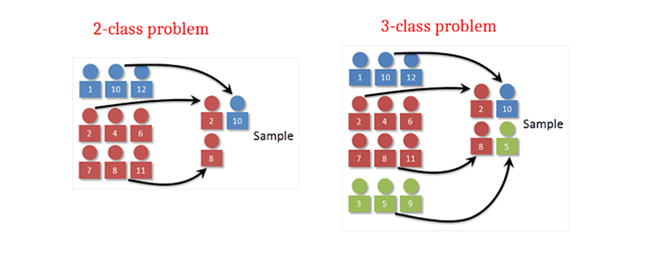
\includegraphics{3.png}

}

\caption{picture}

\end{figure}%

If the model is overfit, we can reduce the polynomial degree, increase
it of underfit. The hyperparameter \texttt{coef0} controls how much the
model is influenced by high-degree vs low-degree of polynomials.

\paragraph{Tips on finding the right
hyperparameter}\label{tips-on-finding-the-right-hyperparameter}

Use grid search multiple times, with each time narrow down the search to
find the optimal hyperparameter.

\subsubsection{7.2.2 Gaussian RBF Kernel}\label{gaussian-rbf-kernel}

To understand about this kernel function, we need to understand about
\textbf{similar features}, which measures how much each instance
resembles a particular \emph{landmark}. Say we have an 1D dataset and
two landmarks at \(x_1=-2\) and \(x_1 = 1\). The similar function will
be the \textbf{RGaussian Radial Basis Function (RBF)} with the equation
is \[
\phi_{\gamma}(\mathbf{x}, \ell) = \exp\left(-\gamma \|\mathbf{x} - \ell\|^2\right)
\] where \(\gamma=0.3\).

This is a bell-shaped function range from 0 (very far from the landmark)
to 1 (at the landmark). Take instance \(x=-1\), it is located 1 distance
from the first landmark and 2 from the second. Therefore, the new
features are \(x_2=\text{exp}(-0.3 \times 1^2) \approx 0.74\) and
\(x_3=\text{exp}(-0.3 \times 2^2) \approx 0.3\).

\begin{figure}[H]

{\centering 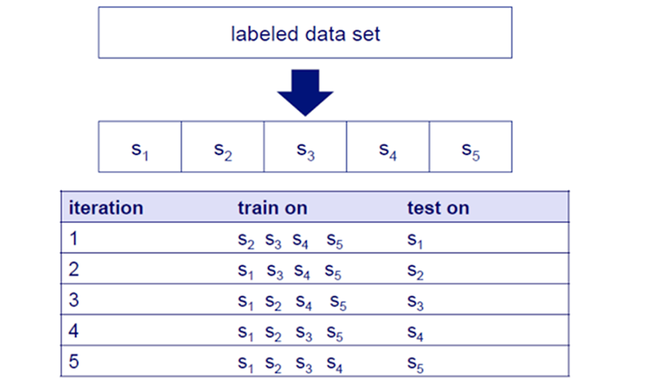
\includegraphics{4.png}

}

\caption{picture}

\end{figure}%

This is just an example, but we create a landmark at the location of all
the instances in the dataset. This brings us back the \textbf{Gaussian
RBF Kernel} where we can do all of this without creating new features.

\begin{Shaded}
\begin{Highlighting}[]
\NormalTok{rbf\_kernel\_svm\_clf }\OperatorTok{=}\NormalTok{ Pipeline([}
\NormalTok{        (}\StringTok{"scaler"}\NormalTok{, StandardScaler()),}
\NormalTok{        (}\StringTok{"svm\_clf"}\NormalTok{, SVC(kernel}\OperatorTok{=}\StringTok{"rbf"}\NormalTok{, gamma}\OperatorTok{=}\DecValTok{5}\NormalTok{, C}\OperatorTok{=}\FloatTok{0.001}\NormalTok{))}
\NormalTok{    ])}
\NormalTok{rbf\_kernel\_svm\_clf.fit(X, y)}
\end{Highlighting}
\end{Shaded}

The hyperparameter gamma \(\gamma\) acts as an regularization that
controls the bell-shaped. Increase \(\gamma\) makes the bell-shaped
curve narrower coz each instance's range of influence is smaller.
Therefore the decision boundary becomes more irregular and wiggling
around individual instances. Conversely, a smaller \(\gamma\) makes the
bell-shaped curve wider, instances have larger range of influence and
the decision boundary is smoother.

\begin{figure}[H]

{\centering 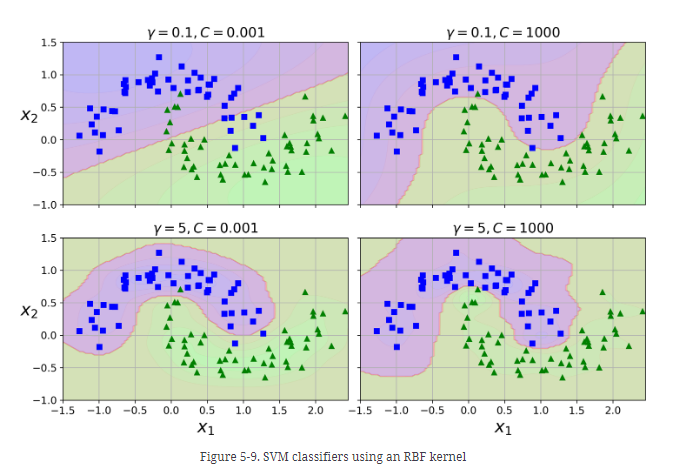
\includegraphics{5.png}

}

\caption{picture}

\end{figure}%

\subsubsection{7.3 SVM Regression}\label{svm-regression}

SVM Regression works inversely to SVM Classification. Instead of trying
to fit the largest possible street between two classes while limiting
the violations, SVM Regression \emph{fit} as many instances as possible
on the street while limiting the violations. The width of the street is
controlled by hyperparameter epsilon \(\epsilon\).

\begin{figure}[H]

{\centering 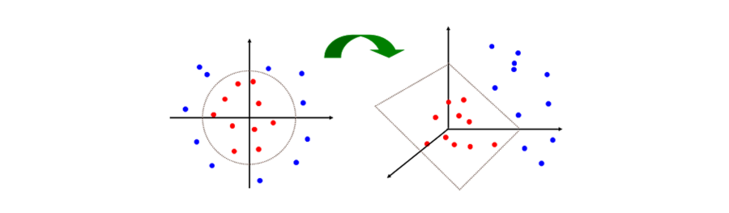
\includegraphics{6.png}

}

\caption{picture}

\end{figure}%

The same things goes for nonlinear SVM.

\subsubsection{7.4 Under the Hood}\label{under-the-hood}

\subsubsection{7.4.1 Decision Function and
Predictions}\label{decision-function-and-predictions}

In a binary classification, the decision function is
\(\mathbf{w}^T\mathbf{x} + b = w_1x_1 + ... + w_nx_n + b\). If the
predicted class \(\hat{y}\) is positive then 1, negative then 0. More
formally, the equation is \[
\hat{y} = \begin{cases}
    0 & \text{if } \mathbf{w}^T \mathbf{x} + b < 0, \\
    1 & \text{if } \mathbf{w}^T \mathbf{x} + b \geq 0
\end{cases}
\]

\begin{figure}[H]

{\centering 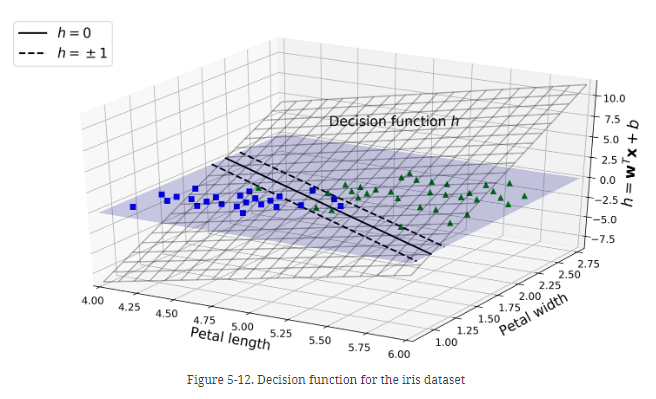
\includegraphics{7.png}

}

\caption{picture}

\end{figure}%

The decision boundary is set to 0, the dashed lines are the points where
the decision function is \(\pm 1\). The dashed lines are parallel to
decision boundary, and formed a margin around it. Training the linear
SVM classifier means to find \(\mathbf{w}\) and \(b\) to make the margin
as wide as possible to avoid margin violations (hard margin) or limiting
them (soft margin).

\subsubsection{7.4.2 Training objective}\label{training-objective}

\begin{figure}[H]

{\centering 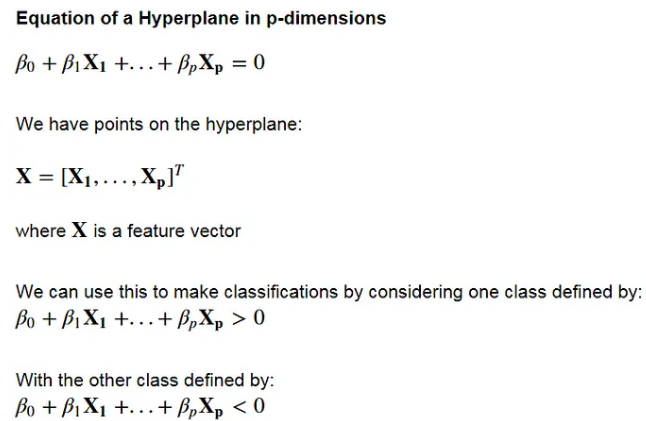
\includegraphics{8.png}

}

\caption{picture}

\end{figure}%

We can see that we need to minimize \(||w||\) to get large margin. We
define \(t^{(i)} = -1\) for negative instances (\(y^{(i)} =0\)) and
\(t^{(i)} = 1\) for positive instances (\(y^{(i)} =1\)), then we can
express the constraint as
\(t^{(i)}(\mathbf{w}^T \mathbf{x}^{(i)} + b) \geq 1\) for all instances.

The objective of hard margin linear SVM classifier is \[
\begin{align*}
\underset{\text{w,b}}{minimize}\quad & \frac{1}{2} \mathbf{w}^T \mathbf{w}  = \frac{1}{2}||w|| \\
\text{subject to} \quad & t^{(i)} \left( \mathbf{w}^T \mathbf{x}^{(i)} + b \right) \geq 1 \quad \text{for } i = 1, 2, \dots, m
\end{align*}
\]

To get the soft margin objective, we need to introduce a \emph{slack
variable} \(\zeta\), which measures how mich instance \(i^{th}\) is
allowed to violate the margin. Now we have 2 conflicting objective, make
\(\zeta\) as small as possible to reduce margin violations, and make
\(||w||\) as small as possible to increase the margin. This is where
hyperparameter \texttt{C} comes in, where it allows us to define the
trade off between the two objectives.

The soft margin linear SVM classifier is \[
\begin{align*}
\underset{\text{w,b},\zeta}{minimize} \quad & \frac{1}{2} \mathbf{w}^T \mathbf{w}  + C\sum_m^{i=1}\zeta^{(i)} \\
\text{subject to} \quad & t^{(i)} \left( \mathbf{w}^T\mathbf{x}^{(i)} + b \right) \geq 1 - \zeta^{(i)} \quad \text{and } \zeta^{(i)} \geq 0 \text{ for } i = 1, 2, \dots, m
\end{align*}
\]

Both hard and soft margin problems are convex quadratic optimizations, I
don't really understand the math so ima skip it :).

\subsubsection{7.4.3 The Dual Problem}\label{the-dual-problem}

We know that the primal problem in SVM is to optimize the margin while
minimizing classification error. \[
\begin{align*}
\underset{\text{w,b},\zeta}{minimize} \quad & \frac{1}{2} \mathbf{w}^T \mathbf{w}  + C\sum_m^{i=1}\zeta^{(i)} \\
\text{subject to} \quad & t^{(i)} \left( \mathbf{w}^T\mathbf{x}^{(i)} + b \right) \geq 1 - \zeta^{(i)} \quad \text{and } \zeta^{(i)} \geq 0 \text{ for } i = 1, 2, \dots, m
\end{align*}
\]

The dual problem derived from the primal problem where dual solution
uses \textbf{Lagrange multipliers} \(\alpha_i\) to determine which
training examples will become support vectors and thus define the
optimal decision boundary.

The dual from of the linear SVM objective is \$\$ \begin{align*}
\underset{\alpha}{minimize} \quad \frac{1}{2}\sum^m_{i=1} \sum^m_{j=1} \alpha^{(i)} \alpha^{(j)} t^{(i)} t^{(j)} \mathbf{x}^{(i)T} \mathbf{x}^{(j)} - \sum^m_{i=1} \alpha^{(i)} \\

\text{subject to } \alpha^{(i)} \geq 0 \text{ for all } i = 1,2,...,m \text{ and } \sum^m_{i=1} \alpha^{(i)}t^{(i)} = 0 
\end{align*} \$\$

Once we find the minimized vector \(\mathbf{\alpha}\) using quadratic
optimizations, we can compute the \(\hat{\mathbf{w}}\) and \(\hat{b}\)
that minimize the primal problem using the following equations \[
\hat{\mathbf{w}} = \sum^m_{i=1}\hat{\alpha}^{(i)}t^{(i)}\mathbf{x}^{(i)} \\
\hat{b} = \frac{1}{n_s} \sum^m_{\underset{\hat{\alpha}^{(i)}> 0}{i=1}} t^{(i)} - \hat{\mathbf{w}}^T\mathbf{x}^{(i)}
\]

where \(n_s\) is the number of support vectors.

The dual problem makes the kernel trick possible, while the primal one
does not.

\subsubsection{7.4.4 Kernelized SVMs}\label{kernelized-svms}

Suppose we want to apply second degree polynomial transformation to a 2D
training set. The second degree polynomial mapping is \[
\phi(\mathbf{x}) = \phi\left(\begin{pmatrix} x_1 \\ x_2 \end{pmatrix}\right) = \begin{pmatrix} x_1^2 \\ \sqrt{2} x_1 x_2 \\ x_2^2 \end{pmatrix}
\]

This is what we normally would do to transform a 2D into 3D, but if we
were to take vectors \(\mathbf{a}\) and \(\mathbf{b}\), and apply this
second degree polynomial mapping and compute the dot product of the
transformed vectors.

\[
\phi(\mathbf{a})^T \phi(\mathbf{b}) = \begin{pmatrix} a_1^2 \\ \sqrt{2} a_1 a_2 \\ a_2^2 \end{pmatrix}^T \begin{pmatrix} b_1^2 \\ \sqrt{2} b_1 b_2 \\ b_2^2 \end{pmatrix} = a_1^2b_1^2 + 2a_1b_1a_2b_2 + a_2^2b_2^2 \\
(a_1b_1 + a_2b_2)^2 = (\begin{pmatrix} a_1 \\ a_2 \end{pmatrix}^T\begin{pmatrix} b_1 \\ b_2 \end{pmatrix})^2 = (\mathbf{a}^T\mathbf{b})^2
\]

The dot product of the transformed vectors = square of the dot product
of the original vectors:
\(\phi(\mathbf{a})^T \phi(\mathbf{b}) = (\mathbf{a}^T\mathbf{b})^2\).

We can conclude that \emph{kernel} is capable of computing the dot
product of \(\phi(\mathbf{a})^T \phi(\mathbf{b})\) based on the original
vectors \(\mathbf{a}\) and \(\mathbf{b}\), without knowing about the
transformation of \(\phi\).

Here are a few common kernels (Géron, 2019).: \[
\begin{align*}
\text{Linear:} \quad & K(\mathbf{a}, \mathbf{b}) = \mathbf{a}^\top \mathbf{b} \\
\text{Polynomial:} \quad & K(\mathbf{a}, \mathbf{b}) = (\gamma \mathbf{a}^\top \mathbf{b} + r)^d \\
\text{Gaussian RBF:} \quad & K(\mathbf{a}, \mathbf{b}) = \exp\left(-\gamma \|\mathbf{a} - \mathbf{b}\|^2\right) \\
\text{Sigmoid:} \quad & K(\mathbf{a}, \mathbf{b}) = \tanh(\gamma \mathbf{a}^\top \mathbf{b} + r)
\end{align*}
\]

\subsection{7.3 Multi-class
classification}\label{multi-class-classification}

Multi-class classification in SVM can be done in 2 ways: one vs all, one
vs one. \#\#\# 7.3.1 One vs all Just like the name suggested, the
samples from the class being trained is viewed as positive, while the
rest is viewed as negative. Say we have classes `0', `1', and `2' in our
dataset. There will be 3 models where model one is `0' vs \{`1' ,`2'\};
model 2 is `1' vs \{`0' ,`2'\}; model 3 is `2' vs \{`0' ,`1'\}.

\begin{figure}[H]

{\centering 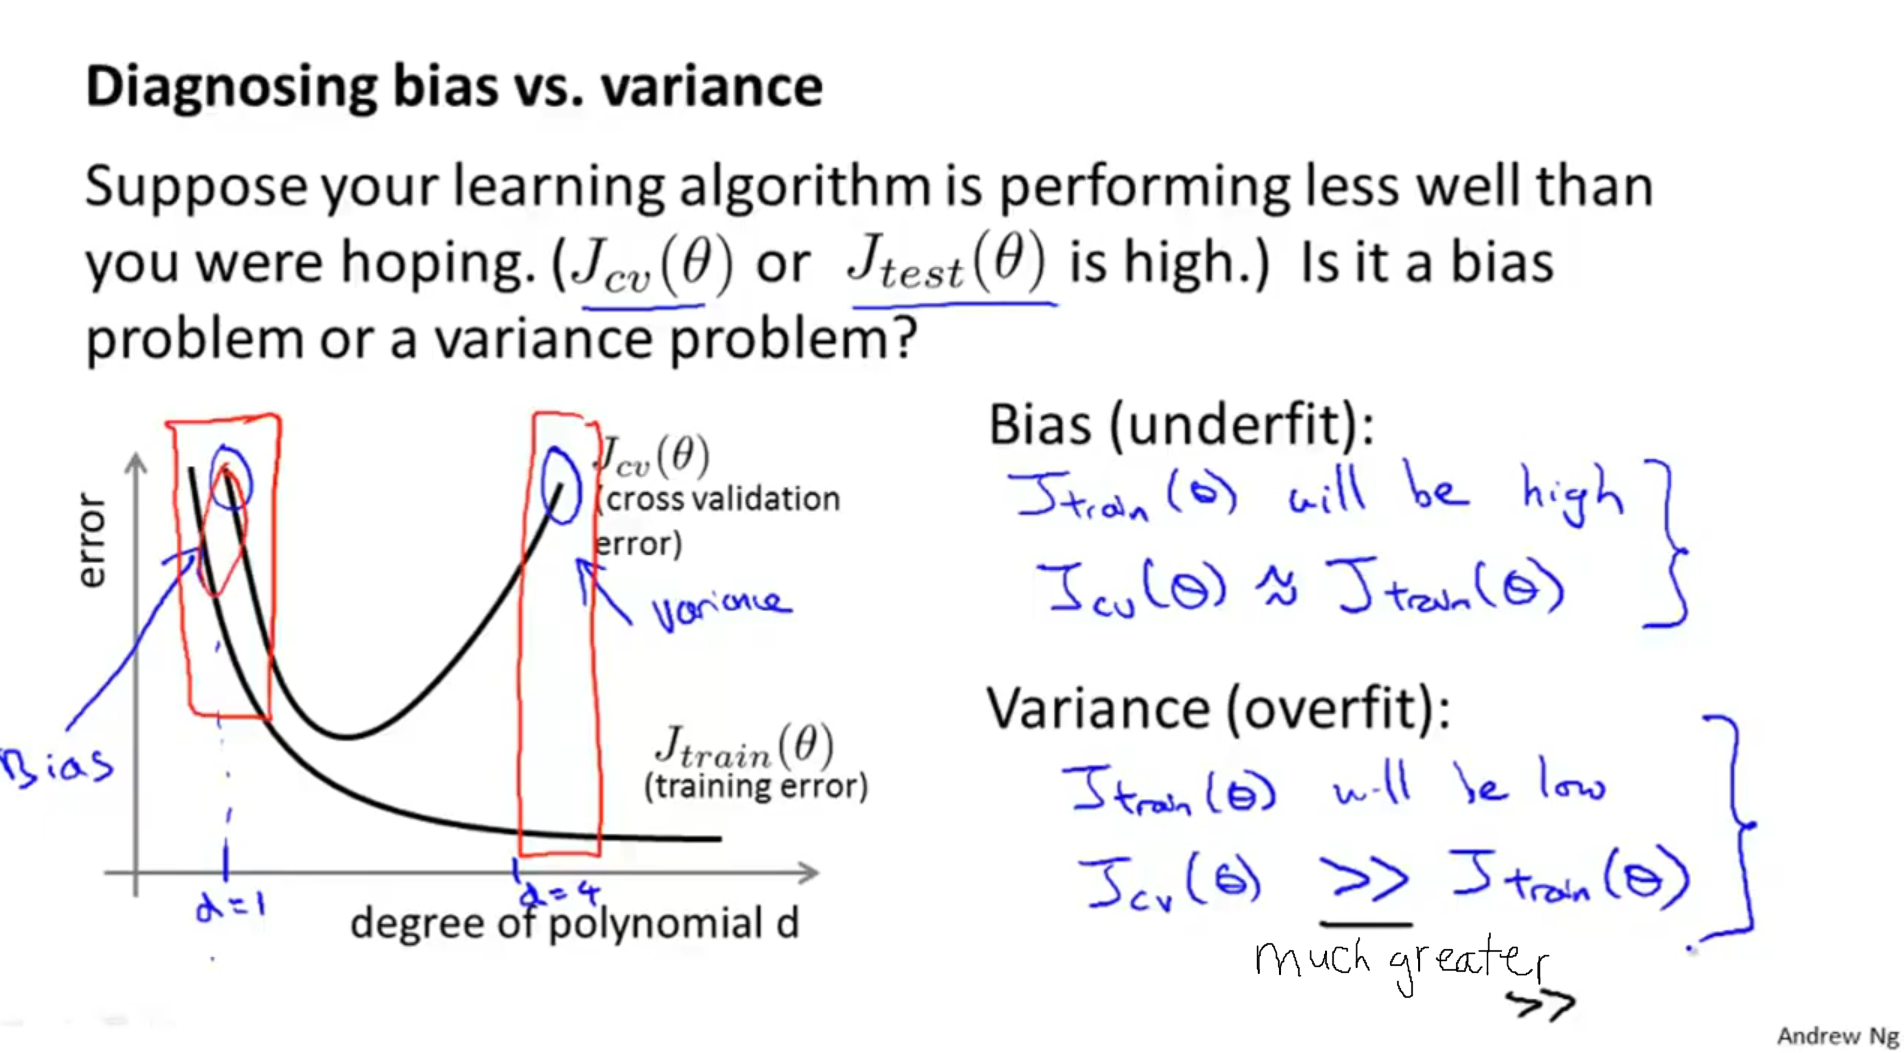
\includegraphics{9.png}

}

\caption{picture}

\end{figure}%

In the prediction phase, the predicted class is determined by the best
model.

\subsubsection{7.3.1 One vs One}\label{one-vs-one}

The SVM algorithm in this case will train multiple binary
classification. Say we have 3 classes (Blue, Green, Red), we would train
3 classifier: Blue vs Green, Blue vs Red, and Green vs Red.

During the prediction phase, the 3 models will vote on the label with
the highest occurrences.

\begin{figure}[H]

{\centering 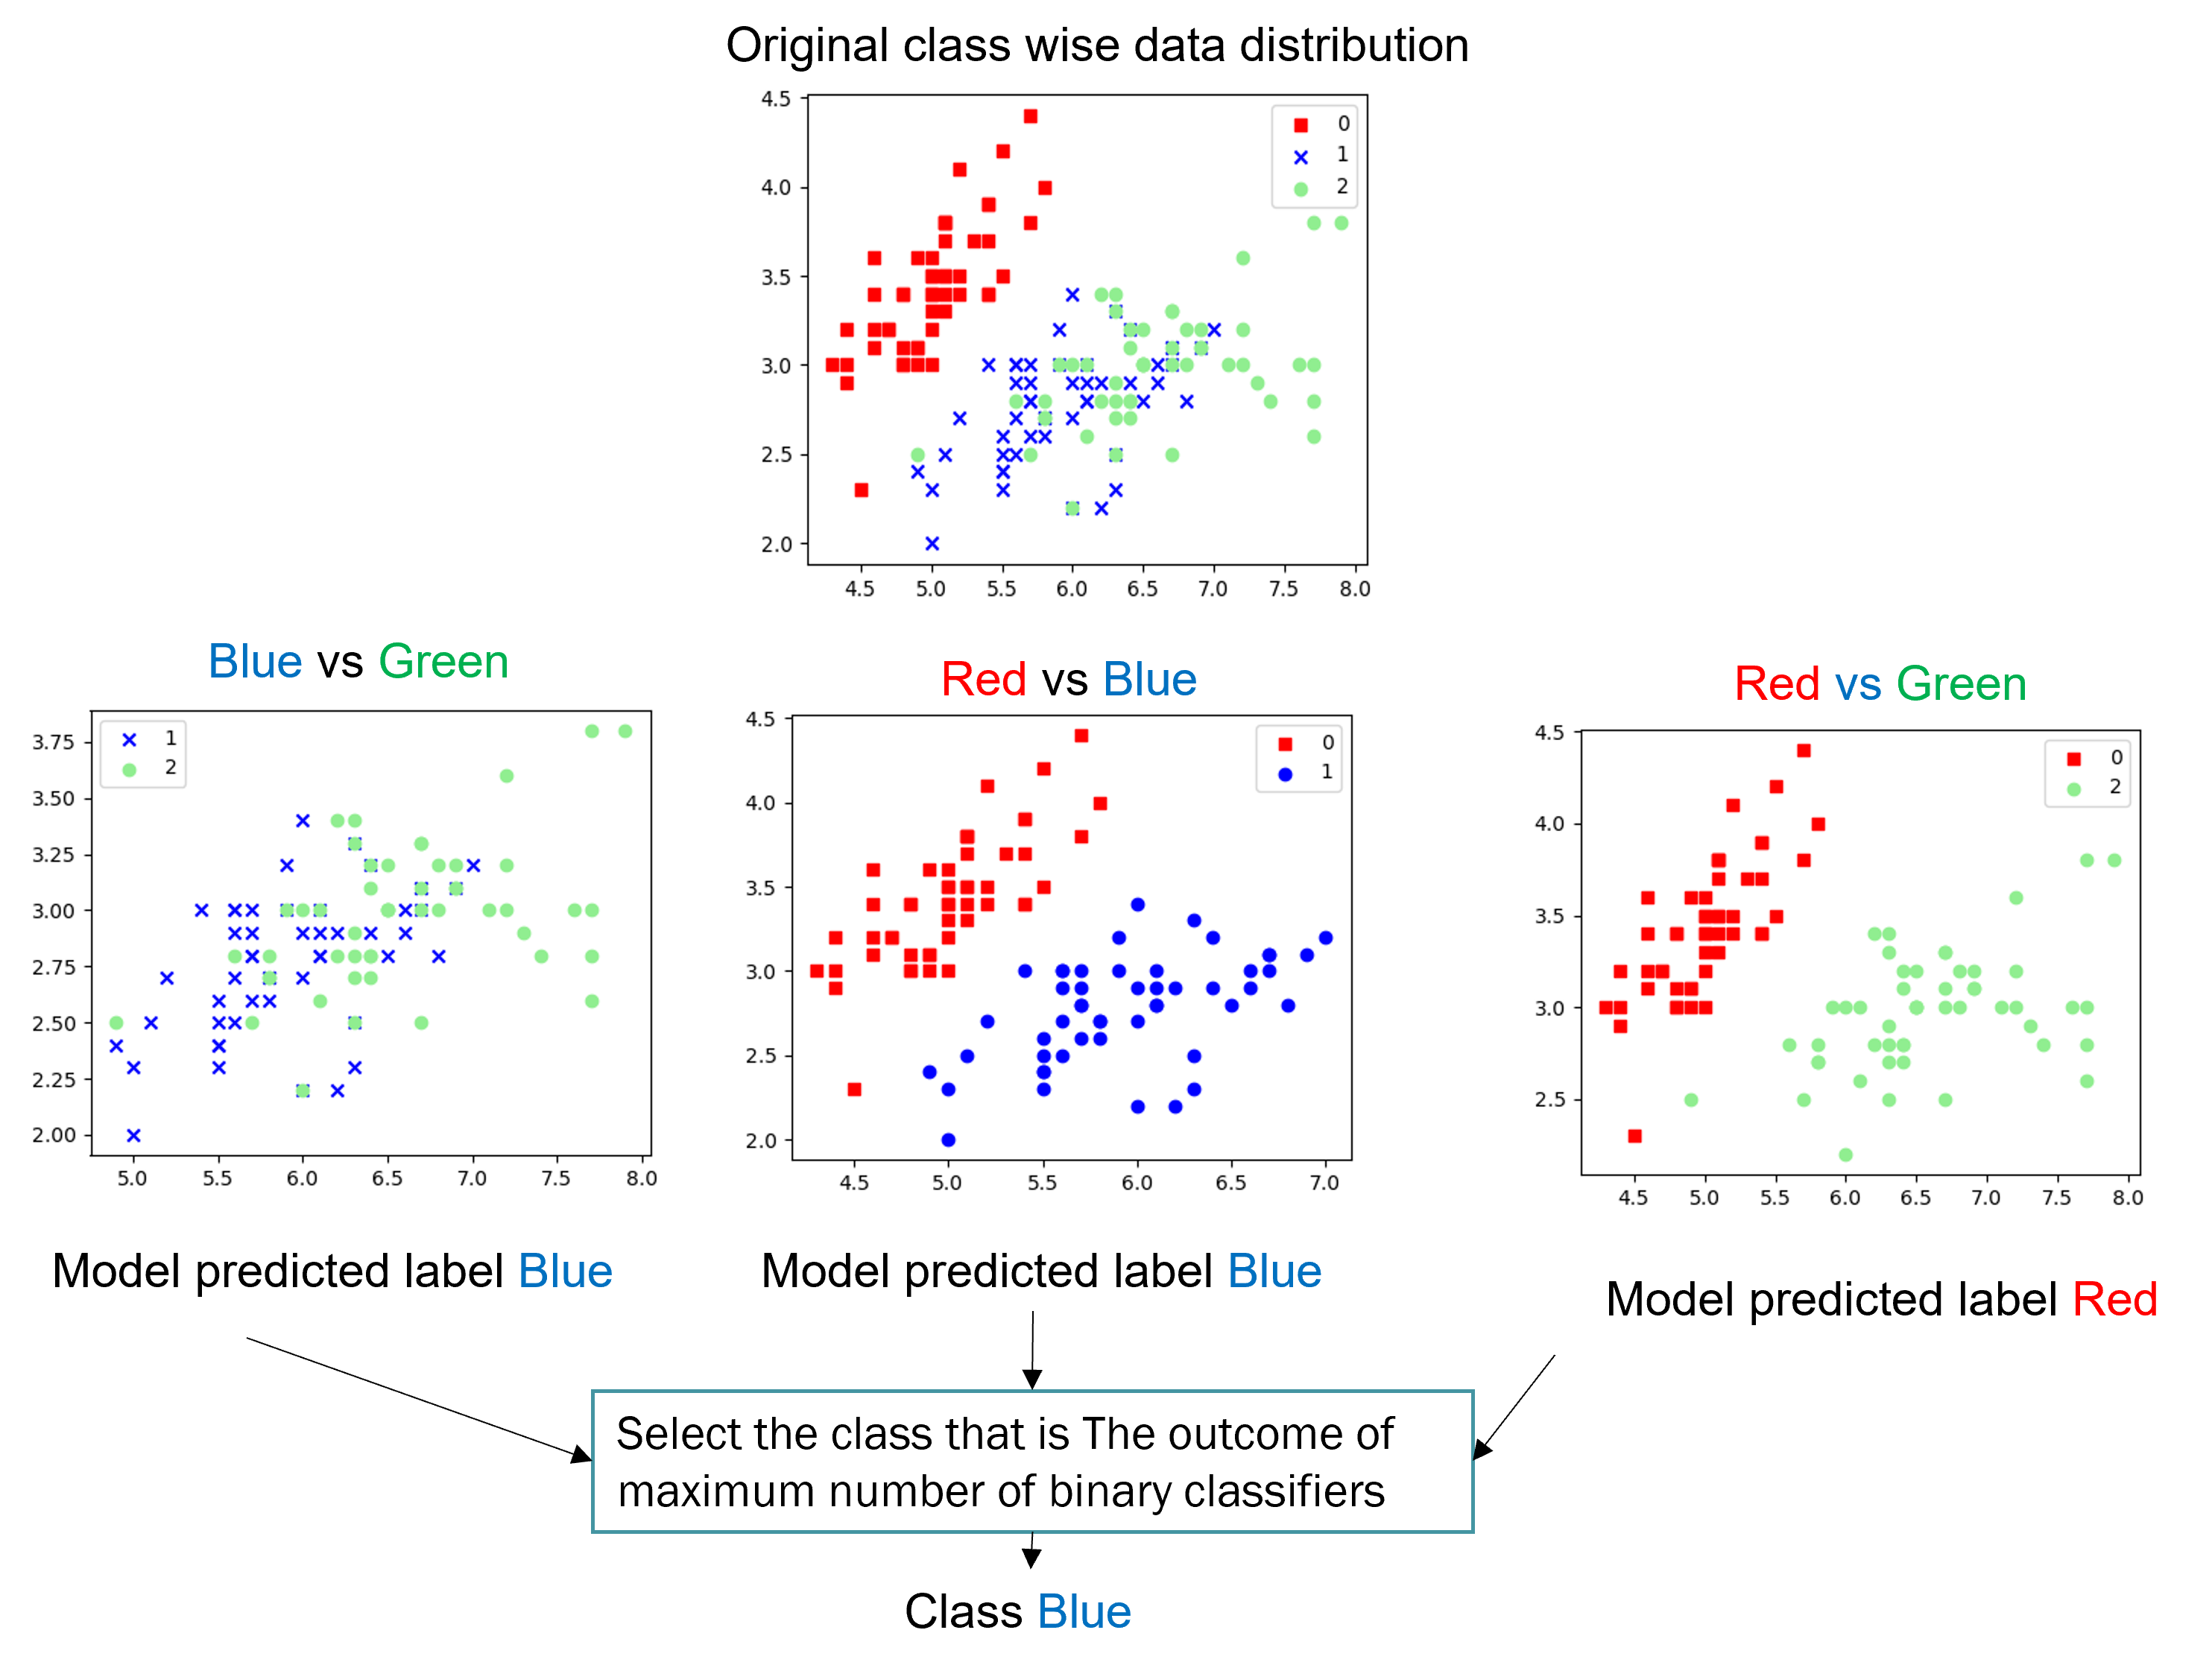
\includegraphics{10.png}

}

\caption{picture}

\end{figure}%

\subsection{7.4 SVM in Python}\label{svm-in-python}

\subsubsection{7.4.1 Linear kernel}\label{linear-kernel}

This is the iris dataset \#\#\#\# Data scaling

\begin{Shaded}
\begin{Highlighting}[]
\ImportTok{from}\NormalTok{ sklearn.preprocessing }\ImportTok{import}\NormalTok{ StandardScaler}
\ImportTok{import}\NormalTok{ seaborn }\ImportTok{as}\NormalTok{ sns}
\ImportTok{from}\NormalTok{ sklearn.model\_selection }\ImportTok{import}\NormalTok{ train\_test\_split}
\ImportTok{import}\NormalTok{ pandas }\ImportTok{as}\NormalTok{ pd}
\ImportTok{import}\NormalTok{ numpy }\ImportTok{as}\NormalTok{ np}
\ImportTok{from}\NormalTok{ sklearn }\ImportTok{import}\NormalTok{ datasets}
\ImportTok{import}\NormalTok{ matplotlib.pyplot }\ImportTok{as}\NormalTok{ plt}

\NormalTok{iris }\OperatorTok{=}\NormalTok{ datasets.load\_iris()}

\CommentTok{\# We\textquotesingle{}ll use the petal length and width only for this analysis}
\NormalTok{X }\OperatorTok{=}\NormalTok{ iris.data}
\NormalTok{y }\OperatorTok{=}\NormalTok{ iris.target}
\CommentTok{\# Place the iris data into a pandas dataframe}
\NormalTok{iris\_df }\OperatorTok{=}\NormalTok{ pd.DataFrame(iris.data, columns}\OperatorTok{=}\NormalTok{iris.feature\_names)}
\NormalTok{X\_train, X\_test, y\_train, y\_test }\OperatorTok{=}\NormalTok{ train\_test\_split(X, y, test\_size}\OperatorTok{=}\FloatTok{.2}\NormalTok{, random\_state}\OperatorTok{=}\DecValTok{0}\NormalTok{)}

\NormalTok{sc }\OperatorTok{=}\NormalTok{ StandardScaler()}

\NormalTok{sc.fit(X\_train)}

\NormalTok{X\_train\_std }\OperatorTok{=}\NormalTok{ sc.transform(X\_train)}
\NormalTok{X\_test\_std }\OperatorTok{=}\NormalTok{ sc.transform(X\_test)}

\NormalTok{plt.figure()}
\NormalTok{iris\_df.hist()}
\NormalTok{plt.suptitle(}\StringTok{"Before scaling"}\NormalTok{)}
\NormalTok{pd.DataFrame(X\_train\_std, columns}\OperatorTok{=}\NormalTok{iris\_df.columns).hist()}
\NormalTok{plt.suptitle(}\StringTok{"After scaling"}\NormalTok{)}
\NormalTok{plt.show()}
\end{Highlighting}
\end{Shaded}

\paragraph{One vs rest}\label{one-vs-rest}

\begin{Shaded}
\begin{Highlighting}[]
\ImportTok{from}\NormalTok{ mlxtend.plotting }\ImportTok{import}\NormalTok{ plot\_decision\_regions}
\ImportTok{from}\NormalTok{ sklearn.decomposition }\ImportTok{import}\NormalTok{ PCA}
\ImportTok{from}\NormalTok{ sklearn.svm }\ImportTok{import}\NormalTok{ SVC}

\NormalTok{pca}\OperatorTok{=}\NormalTok{PCA(n\_components}\OperatorTok{=}\DecValTok{2}\NormalTok{)}
\NormalTok{reduced\_data\_train}\OperatorTok{=}\NormalTok{pca.fit\_transform(X\_train\_std)}
\NormalTok{reduced\_data\_test}\OperatorTok{=}\NormalTok{pca.transform(X\_test\_std)}
\NormalTok{classifier}\OperatorTok{=}\NormalTok{SVC(kernel}\OperatorTok{=}\StringTok{\textquotesingle{}linear\textquotesingle{}}\NormalTok{, random\_state}\OperatorTok{=}\DecValTok{0}\NormalTok{, gamma}\OperatorTok{=}\FloatTok{.10}\NormalTok{, C}\OperatorTok{=}\FloatTok{1.0}\NormalTok{).fit(reduced\_data\_train,y\_train)}
\NormalTok{plt.figure(figsize}\OperatorTok{=}\NormalTok{(}\DecValTok{10}\NormalTok{,}\DecValTok{3}\NormalTok{))}

\NormalTok{classifier}\OperatorTok{=}\NormalTok{SVC(kernel}\OperatorTok{=}\StringTok{"linear"}\NormalTok{, random\_state}\OperatorTok{=}\DecValTok{0}\NormalTok{, gamma}\OperatorTok{=}\FloatTok{.10}\NormalTok{, C}\OperatorTok{=}\FloatTok{1.0}\NormalTok{,decision\_function\_shape}\OperatorTok{=}\StringTok{\textquotesingle{}ovr\textquotesingle{}}\NormalTok{).fit(reduced\_data\_train,y\_train)}
\CommentTok{\# Plot decision boundary}
\NormalTok{plot\_decision\_regions(reduced\_data\_test, y\_test, clf}\OperatorTok{=}\NormalTok{classifier, legend}\OperatorTok{=}\DecValTok{2}\NormalTok{)}
\NormalTok{plt.legend(ncol}\OperatorTok{=}\DecValTok{3}\NormalTok{)}
\NormalTok{plt.axis(}\StringTok{"off"}\NormalTok{)}
\NormalTok{plt.show()}
\end{Highlighting}
\end{Shaded}

\paragraph{One vs One}\label{one-vs-one-1}

\begin{Shaded}
\begin{Highlighting}[]
\ImportTok{from}\NormalTok{ mlxtend.plotting }\ImportTok{import}\NormalTok{ plot\_decision\_regions}
\NormalTok{plt.figure(figsize}\OperatorTok{=}\NormalTok{(}\DecValTok{10}\NormalTok{,}\DecValTok{3}\NormalTok{))}

\NormalTok{classifier}\OperatorTok{=}\NormalTok{SVC(kernel}\OperatorTok{=}\StringTok{"linear"}\NormalTok{, random\_state}\OperatorTok{=}\DecValTok{0}\NormalTok{, gamma}\OperatorTok{=}\FloatTok{.10}\NormalTok{, C}\OperatorTok{=}\FloatTok{1.0}\NormalTok{,decision\_function\_shape}\OperatorTok{=}\StringTok{\textquotesingle{}ovo\textquotesingle{}}\NormalTok{).fit(reduced\_data\_train,y\_train)}
\CommentTok{\# Plot decision boundary}
\NormalTok{plot\_decision\_regions(reduced\_data\_test, y\_test, clf}\OperatorTok{=}\NormalTok{classifier, legend}\OperatorTok{=}\DecValTok{2}\NormalTok{)}
\NormalTok{plt.legend(ncol}\OperatorTok{=}\DecValTok{3}\NormalTok{)}
\NormalTok{plt.axis(}\StringTok{"off"}\NormalTok{)}
\NormalTok{plt.show()}
\end{Highlighting}
\end{Shaded}

\subsubsection{7.4.2 Kernel trick}\label{kernel-trick}

\paragraph{Regularisation}\label{regularisation}

\begin{Shaded}
\begin{Highlighting}[]
\ImportTok{from}\NormalTok{ cuml.svm }\ImportTok{import}\NormalTok{ SVC}
\ImportTok{from}\NormalTok{ cuml.model\_selection }\ImportTok{import}\NormalTok{ GridSearchCV}

\CommentTok{\# parameters to search}
\NormalTok{param\_grid }\OperatorTok{=}\NormalTok{ \{}
    \StringTok{\textquotesingle{}C\textquotesingle{}}\NormalTok{: [}\FloatTok{0.1}\NormalTok{, }\DecValTok{1}\NormalTok{, }\DecValTok{10}\NormalTok{, }\DecValTok{100}\NormalTok{],          }\CommentTok{\# Regularization parameter}
    \StringTok{\textquotesingle{}kernel\textquotesingle{}}\NormalTok{: [}\StringTok{\textquotesingle{}linear\textquotesingle{}}\NormalTok{, }\StringTok{\textquotesingle{}rbf\textquotesingle{}}\NormalTok{, }\StringTok{\textquotesingle{}poly\textquotesingle{}}\NormalTok{],  }\CommentTok{\# Kernel types}
    \StringTok{\textquotesingle{}degree\textquotesingle{}}\NormalTok{: [}\DecValTok{2}\NormalTok{, }\DecValTok{3}\NormalTok{, }\DecValTok{4}\NormalTok{],             }\CommentTok{\# Degree for the polynomial kernel}
    \StringTok{\textquotesingle{}gamma\textquotesingle{}}\NormalTok{: [}\StringTok{\textquotesingle{}scale\textquotesingle{}}\NormalTok{, }\StringTok{\textquotesingle{}auto\textquotesingle{}}\NormalTok{],      }\CommentTok{\# Kernel coefficient}
\NormalTok{\}}
\NormalTok{svc }\OperatorTok{=}\NormalTok{ SVC()}
\NormalTok{grid\_search }\OperatorTok{=}\NormalTok{ GridSearchCV(svc, param\_grid, cv}\OperatorTok{=}\DecValTok{5}\NormalTok{, scoring}\OperatorTok{=}\StringTok{\textquotesingle{}accuracy\textquotesingle{}}\NormalTok{)}
\NormalTok{grid\_search.fit(X\_train, y\_train)}

\CommentTok{\# Display the best hyperparameters}
\BuiltInTok{print}\NormalTok{(}\StringTok{"Best hyperparameters: "}\NormalTok{, grid\_search.best\_params\_)}
\BuiltInTok{print}\NormalTok{(}\StringTok{"Best score: "}\NormalTok{, grid\_search.best\_score\_)}
\end{Highlighting}
\end{Shaded}

We can see that with grid search, we found the best hyperparameters and
score of our dataset.

\section{Week 8: Nonlinear models (KNN and
DT)}\label{week-8-nonlinear-models-knn-and-dt}

\subsection{8.1 K-Nearest Neighbors
(KNN)}\label{k-nearest-neighbors-knn}

The information below is summarized from IBM (2024). People often
mistake KNN with unsupervised learning, KNN is in fact an
\textbf{supervised learning} algorithm, and can be used both for
regression and classification, but mostly classification.

\subsubsection{Classification problem}\label{classification-problem}

The class label is assigned based on the majority of the given data
points surrounding it.

\begin{figure}[H]

{\centering 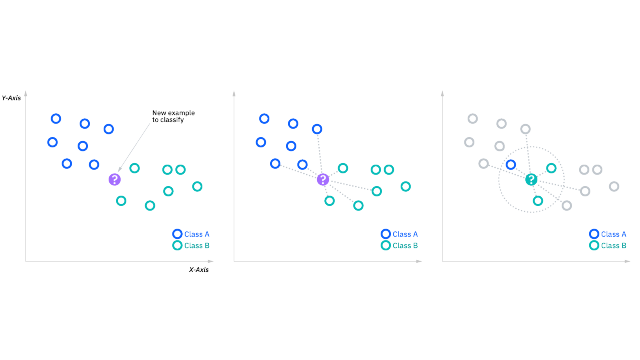
\includegraphics{11.png}

}

\caption{picture}

\end{figure}%

\subsubsection{Regression problem}\label{regression-problem}

Regression uses a similar concepts to classification, but regression
average the k nearest neighbors to make prediction. One is continuous
value, the other is discrete value.

Say \(K=5\), and the 5 closest neighbors are 4.2, 3.8, 5.0, 4.7, 4.5.
The prediction will be \(\frac{4.2+3.8+5.0+4.7+4.5}{5}=4.44\).

\subsubsection{Compute Distance}\label{compute-distance}

Before the algorithm classifies things, it needs to compute the
distance. In other words, there needs to be some metrics like Euclidean
or Manhattan or whatever to measure how close the other data points are
to our query point (IBM, 2024).

\subsubsection{Best number of neighbours
(K)}\label{best-number-of-neighbours-k}

We need to choose the most optimal number of \(K\) in order for our
classification to perform well. Choosing lower number of \(k\), meaning
focusing on the close region, this has the higher change of overfitting.
The opposite can be said for high \(k\), this can cause underfitting. We
can use grid search to search for the optimal number of \(k\).

\begin{figure}[H]

{\centering 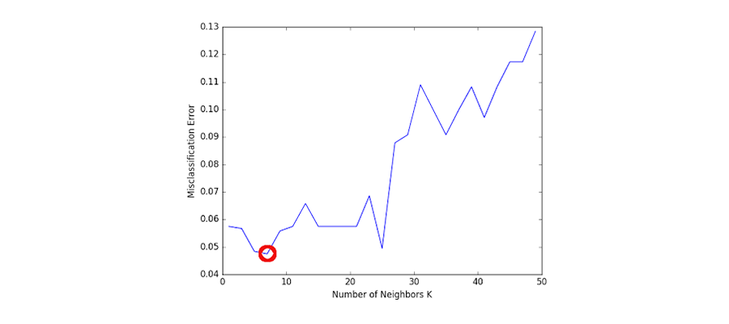
\includegraphics{12.png}

}

\caption{picture}

\end{figure}%

\subsection{8.2 Decision trees}\label{decision-trees}

The information below is from Géron, A. (2019).

The text discusses the training, visualizing, and making predictions
with Decision Trees. Then the CART training algorithm, and how to
regularize trees for regression tasks. Finally is on the limitations of
Decision Trees.

\subsubsection{Training and Visualizing a Decision
Tree}\label{training-and-visualizing-a-decision-tree}

\begin{Shaded}
\begin{Highlighting}[]
\ImportTok{from}\NormalTok{ sklearn.datasets }\ImportTok{import}\NormalTok{ load\_iris}
\ImportTok{from}\NormalTok{ sklearn.tree }\ImportTok{import}\NormalTok{ DecisionTreeClassifier}

\NormalTok{iris }\OperatorTok{=}\NormalTok{ load\_iris()}
\NormalTok{X }\OperatorTok{=}\NormalTok{ iris.data[:, }\DecValTok{2}\NormalTok{:] }\CommentTok{\# petal length and width}
\NormalTok{y }\OperatorTok{=}\NormalTok{ iris.target}

\NormalTok{tree\_clf }\OperatorTok{=}\NormalTok{ DecisionTreeClassifier(max\_depth}\OperatorTok{=}\DecValTok{2}\NormalTok{)}
\NormalTok{tree\_clf.fit(X, y)}
\end{Highlighting}
\end{Shaded}

\begin{Shaded}
\begin{Highlighting}[]
\ImportTok{from}\NormalTok{ sklearn.tree }\ImportTok{import}\NormalTok{ export\_graphviz}

\NormalTok{export\_graphviz(}
\NormalTok{        tree\_clf,}
\NormalTok{        out\_file}\OperatorTok{=}\StringTok{"iris\_tree.dot"}\NormalTok{,}
\NormalTok{        feature\_names}\OperatorTok{=}\NormalTok{iris.feature\_names[}\DecValTok{2}\NormalTok{:],}
\NormalTok{        class\_names}\OperatorTok{=}\NormalTok{iris.target\_names,}
\NormalTok{        rounded}\OperatorTok{=}\VariableTok{True}\NormalTok{,}
\NormalTok{        filled}\OperatorTok{=}\VariableTok{True}
\NormalTok{    )}
\end{Highlighting}
\end{Shaded}

\begin{figure}[H]

{\centering 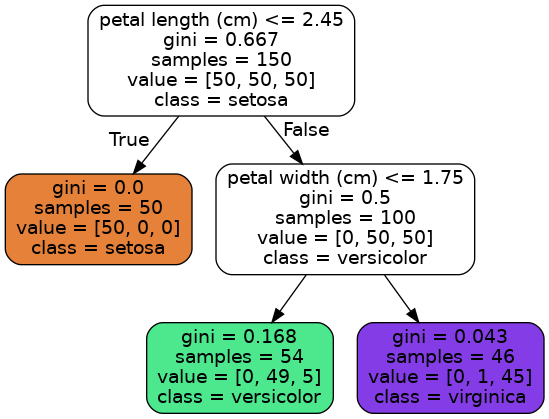
\includegraphics{iris_tree.png}

}

\caption{picture}

\end{figure}%

\subsubsection{Making prediction}\label{making-prediction}

Suppose there is a iris flower, and the algorithm wants to classify it.
Start off with the \emph{root node} (depth 0, top node): this node asks
if \(\text{petal length} \leq 2.45\), if yes then move down the leaf
node (node that doesn't have child node) or the root's left child node
(depth 1, left), which classifies the iris flower as \texttt{setosa}.

If say find another flower, but this time
\(\text{petal length} > 2.45\), the algorithm goes down to right child
node (depth 1, right), which is not a leaf node. This right node asks
\(\text{petal width} \leq 1.75\)? If yes then the class is
\texttt{versicolor}, no then \texttt{virginica}.

A node's \texttt{sample} tells us how many training instaces it applies
to. Right child node (depth 1) has 100 instances where
\(\text{petal length} > 2.45\). In those 100, 54 has a
\(\text{petal width} < 1.75\).

The \texttt{value} shows the classification of training instaces. Take
the botton right node, there are 0 \emph{setosa}, 1 \emph{versicolor},
and 45 \emph{virginica}. It made 1 mistake. The \texttt{gini} measures
the purity of a node, with 0 being the purest. The formula is \[
G_i = 1 - \sum_{k=1}^np_{i,k^2}
\] where \(p_{i,k^2}\) is the ratio of class \(k\) instances among the
training instances in \(i^{th}\) node.

We can calculate the purity for bottom left node:
\(1-(0/46)^2 - (1/46)^2 - (45/46)^2 = 0.0425 = 0.043\)

Note: sklearn uses \textbf{CART} algorithm, whcih produces only binary
trees. (yes/no answer), however algorithm like \textbf{ID3} produces
nodes that have more than 2 children.

This picture represents the decision tree's boundaries

\begin{figure}[H]

{\centering 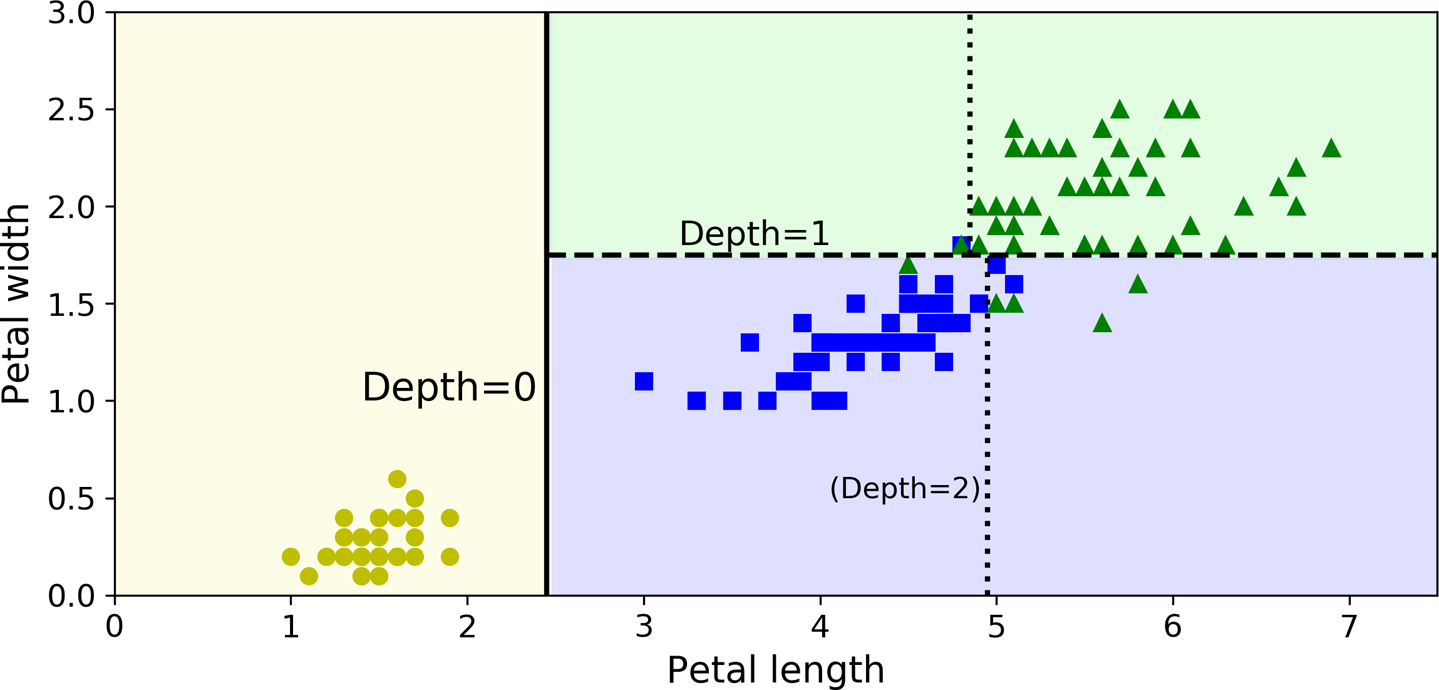
\includegraphics{13.png}

}

\caption{picture}

\end{figure}%

On the left hand where depth 0 shows a thick line because the
\emph{gini} is pure. For the right hand side where the \emph{gini} is
impure, so there are more splits. Since we can clearly intepret the
decisions from Decision Trees, we can say this model is \textbf{white
box model}. Models like Random Forest and NN are \textbf{black box
models} because those models are hard to intepret the reasons for their
predictions.

\subsubsection{Estimating Class
Probabilities}\label{estimating-class-probabilities}

A Decision Tree can estimate the probability of what class an instance
belongs to by traversing the tree to the find leaf node for that
instance. For example, take a flower where petals are 5cm long and 1.5cm
wide. Looking at the decision boundary, we can see that this flower is
versicolor. It belongs to depth 1 where the probabilities for Iris
setosa (0/54) is 0\%, Iris versicolor (49/54) is 90.7\%, and Iris
virginica (5/54) is 9.3\%.

\begin{Shaded}
\begin{Highlighting}[]
\NormalTok{display(tree\_clf.predict\_proba([[}\DecValTok{5}\NormalTok{, }\FloatTok{1.5}\NormalTok{]]))}
\NormalTok{display(tree\_clf.predict([[}\DecValTok{5}\NormalTok{, }\FloatTok{1.5}\NormalTok{]]))}
\end{Highlighting}
\end{Shaded}

Take another example with petals 6cm long and 2cm wide, it would be
virginica.

\begin{Shaded}
\begin{Highlighting}[]
\NormalTok{display(tree\_clf.predict\_proba([[}\DecValTok{6}\NormalTok{, }\DecValTok{2}\NormalTok{]]))}
\NormalTok{display(tree\_clf.predict([[}\DecValTok{6}\NormalTok{, }\DecValTok{2}\NormalTok{]]))}
\end{Highlighting}
\end{Shaded}

\subsubsection{The CART Training
Algorithm}\label{the-cart-training-algorithm}

Classification and Regression Tree or CART algorithm train Decision
Trees (aka ``growing'' trees). The algorithm works by splitting into two
subsets using a single feature \(k\) and a threshold \(t_k\)
(\(\text{petal length} \leq 2.45\)). To choose the pair (\(k\) and
\(t_k\)), it searches for the pair that gives the purest subsets. This
process repeats itself until it reaches the maximum depth
(hyperparameter \texttt{max\_depth}), or can not find a split to reduce
the impurity. There are a few other hyperparameters. The formula for
CART with the cost function that the algorithm tries to minimize is: \[
J(k,t_k) = \frac{m_{\text{left}}}{m}G_{\text{left}} + \frac{m_{\text{right}}}{m}G_{\text{right}}
\] where - \(G_{\text{left/right}}\) measures the impurity of the
left/right subset - \(m_{\text{left/right}}\) is the number of instances
in the left/right subset

This is a greedy algorithm where it searches for the lowest possible
impurity split from top down, which can lead to overfitting.

\subsubsection{Gini Impurity or Entropy}\label{gini-impurity-or-entropy}

Impurity and Entropy are two measurement for Gini. A set's entropy is
zero when it contains instances of only one class. The formula for
entropy is: \[
H_i = -\sum^n_{k=1, p_{i,k^{\neq 0}}}p_{i,k}log_2(p_{i,k})
\] In depth 2, the entropy is
\(–(49/54) log2 (49/54) – (5/54) log2 (5/54) ≈ 0.445\).

Choosing between one of the 2 is not really imporant.

\subsubsection{Regularization
Hyperparameters}\label{regularization-hyperparameters}

Decision Tree is a \emph{nonparametric model}, which means there are
less default parameters determined, and we need to define them. Unlike
\emph{parametric model} like Linear Regression where there are many
default parameters. Since Decision Tree is a nonparametric model, and
the model is trying to find the lowest possible impurity split from top
down, this can cause overfitting.

Hyperparameters are regularization: \texttt{max\_depth} means max split.
In DecisionTreeClassifier we have \texttt{min\_samples\_split} = minimum
number of samples a node must have before split;
\texttt{min\_samples\_leaf} = minimum number of samples a leaf must
have; \texttt{min\_weight\_fraction\_leaf} = same as
\texttt{min\_samples\_leaf} but expressed as fraction of the total
number of weighted instaces. More on the website\textgreater{}

\subsubsection{Regression}\label{regression}

\begin{Shaded}
\begin{Highlighting}[]
\ImportTok{from}\NormalTok{ sklearn.tree }\ImportTok{import}\NormalTok{ DecisionTreeRegressor}

\NormalTok{tree\_reg }\OperatorTok{=}\NormalTok{ DecisionTreeRegressor(max\_depth}\OperatorTok{=}\DecValTok{2}\NormalTok{)}
\NormalTok{tree\_reg.fit(X, y)}
\end{Highlighting}
\end{Shaded}

\begin{figure}[H]

{\centering 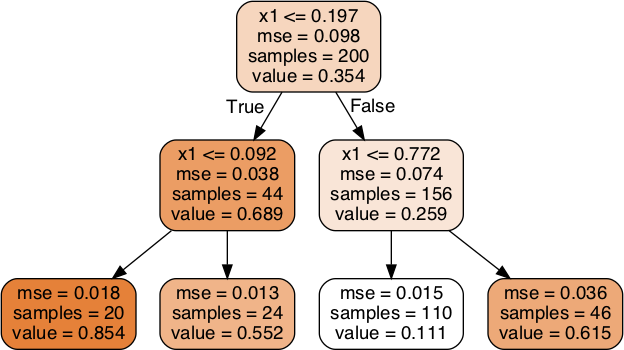
\includegraphics{14.png}

}

\caption{picture}

\end{figure}%

Now instead of predicting a class for each node, it predicts a value.
Say a instance \(x_1=0.6\), and transverse starting from the root node,
we reach a leaf node that predicts \texttt{value=0.111}. This prediction
is the average target value of 110 \texttt{samples} in the leaf node,
and the \texttt{mse} is 0.015 over the 110 instances.

The predicted value for each region is always the average target value
of the instances in that region.

\begin{figure}[H]

{\centering 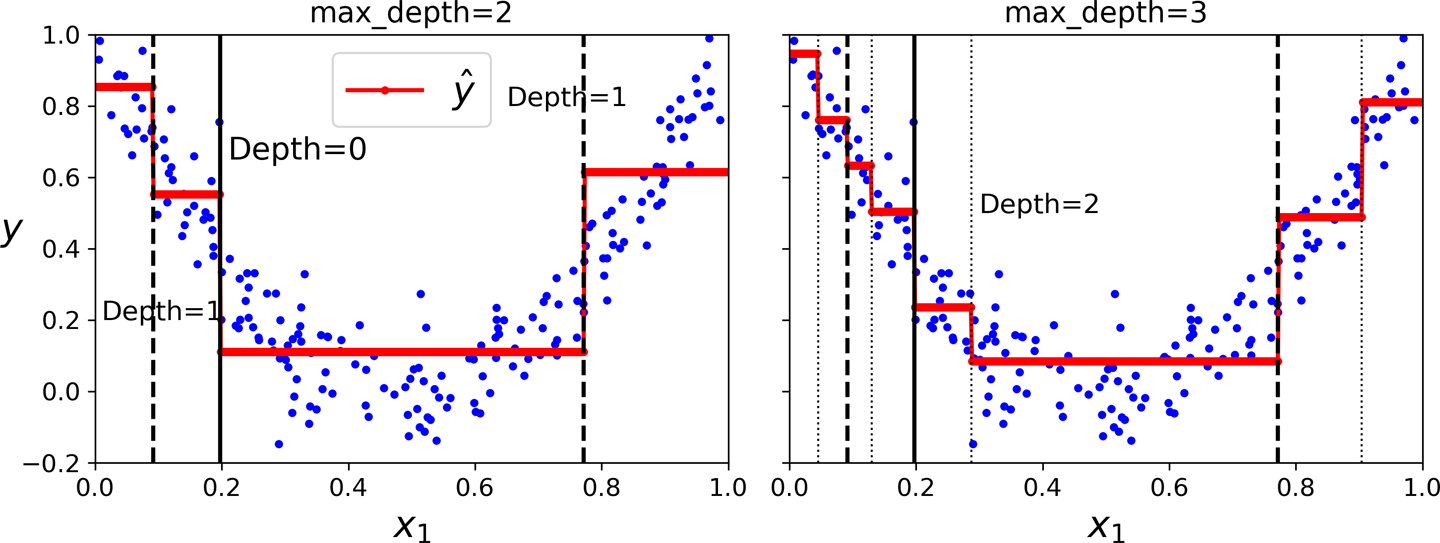
\includegraphics{15.png}

}

\caption{picture}

\end{figure}%

The CART algorithm minimizes MSE instead of purity. The formula is: \[
J(k,t_k) = \frac{m_{\text{left}}}{m}\text{MSE}_{\text{left}} + \frac{m_{\text{right}}}{m}\text{MSE}_{\text{right}}
\] where -
\(\text{MSE}_{\text{node}} = \sum_{i \in \text{node}}(\hat{y}_{\text{node}} - y^{(i)})^2\)
-
\(\hat{y}_{\text{node}} = \frac{1}{m_{\text{node}}}\sum_{i \in \text{node}}y^{(i)}\)

Just like classification, regression can overfit if no restriction is
put into place.

\begin{figure}[H]

{\centering 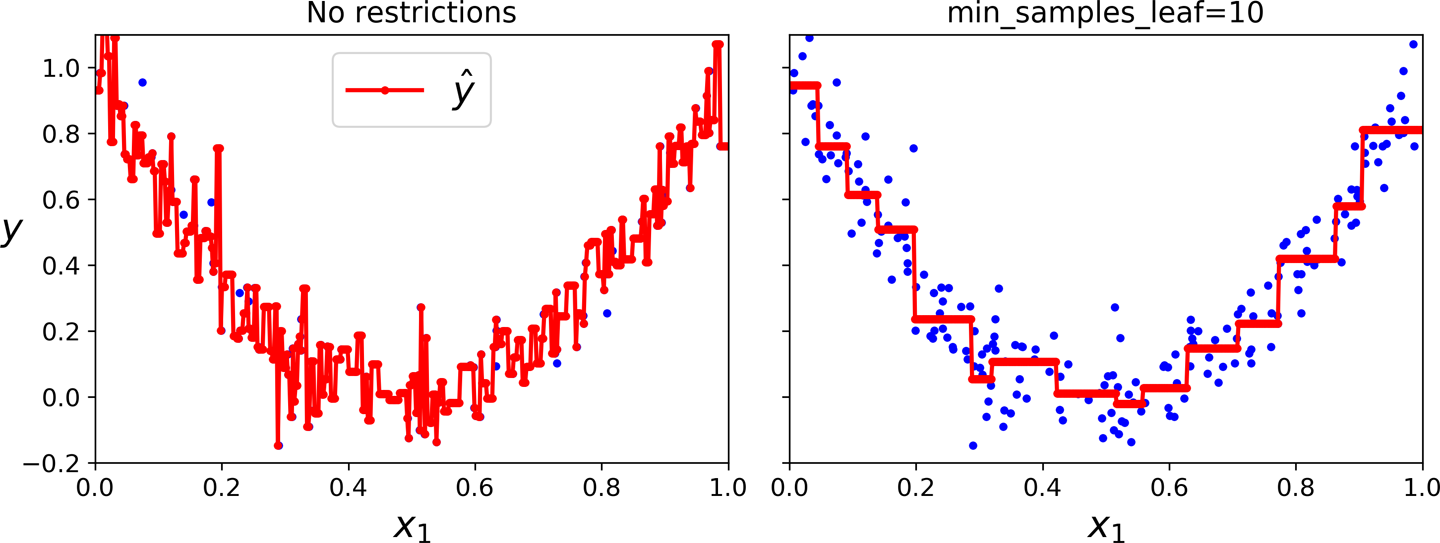
\includegraphics{16.png}

}

\caption{picture}

\end{figure}%

\subsubsection{Instability}\label{instability}

One of the thing is that Decision Tree loves orthogonal decision
boundaries (all splits are perpendicular to an axis). This makes the
boundary unnecessarily convoluted and may not generalize well.

\begin{figure}[H]

{\centering 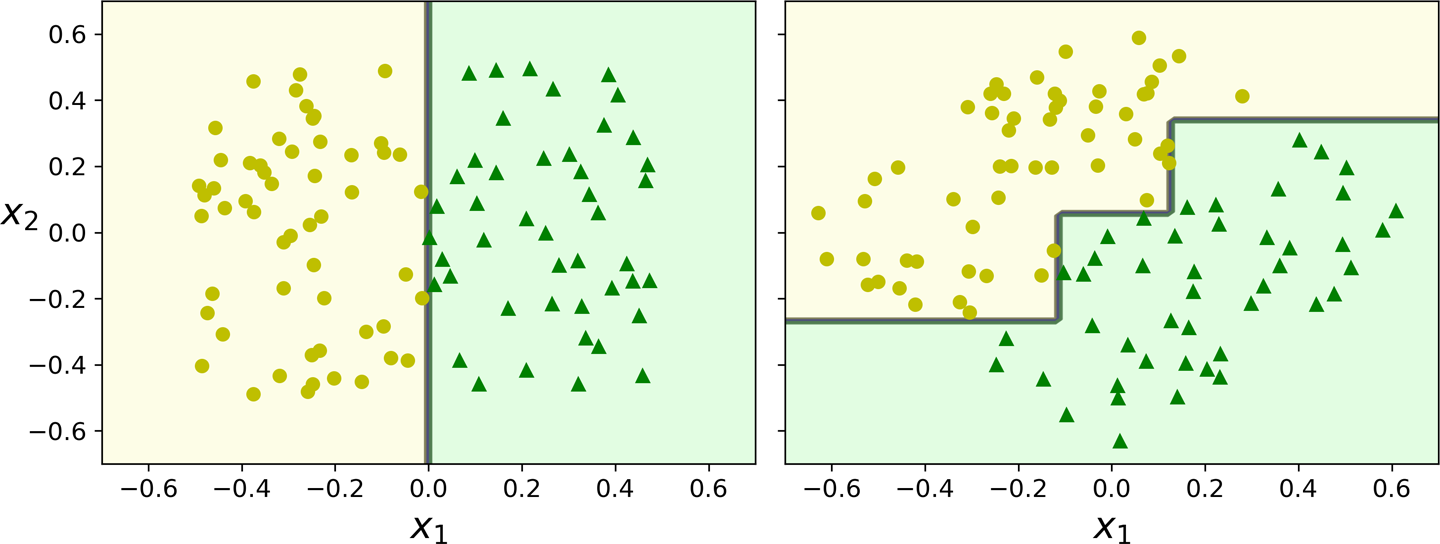
\includegraphics{17.png}

}

\caption{picture}

\end{figure}%

Another thing is that Decision Tree is very sensitive to small
variations in the training data. If we were to remove some extreme
value, the model will look vastly different. Even with the same training
set, the output decision boundary can be different unless we set
\texttt{random\_state}. This can be solve using \textbf{Random Forest}
(Géron, 2019).

\subsubsection{Post and Pre-Pruning}\label{post-and-pre-pruning}

The information below is from Anand (2020).

Pruning just means to remove braches of the decision tree to overcome
overfitting. This can be achieved by post and pre-pruning.

\paragraph{Post Pruning (Backward
pruning)}\label{post-pruning-backward-pruning}

This technique is used after constructing the decision tree. We will
control the \texttt{max\_depth} and \texttt{min\_samples\_split} using
\texttt{cost\_complexity\_pruning}. We will be using the breast\_cancer
dataset.

\begin{Shaded}
\begin{Highlighting}[]
\ImportTok{import}\NormalTok{ numpy }\ImportTok{as}\NormalTok{ np}
\ImportTok{import}\NormalTok{ pandas }\ImportTok{as}\NormalTok{ pd}
\ImportTok{import}\NormalTok{ matplotlib.pyplot }\ImportTok{as}\NormalTok{ plt}
\ImportTok{import}\NormalTok{ seaborn }\ImportTok{as}\NormalTok{ sns}
\ImportTok{from}\NormalTok{ sklearn }\ImportTok{import}\NormalTok{ tree}
\ImportTok{from}\NormalTok{ sklearn.metrics }\ImportTok{import}\NormalTok{ accuracy\_score}
\ImportTok{from}\NormalTok{ sklearn.datasets }\ImportTok{import}\NormalTok{ load\_breast\_cancer}
\ImportTok{from}\NormalTok{ sklearn.model\_selection }\ImportTok{import}\NormalTok{ train\_test\_split}
\ImportTok{from}\NormalTok{ sklearn.tree }\ImportTok{import}\NormalTok{ DecisionTreeClassifier}
\end{Highlighting}
\end{Shaded}

\begin{Shaded}
\begin{Highlighting}[]
\NormalTok{X,y}\OperatorTok{=}\NormalTok{load\_breast\_cancer(return\_X\_y}\OperatorTok{=}\VariableTok{True}\NormalTok{)}
\NormalTok{X\_train,X\_test,y\_train,y\_test}\OperatorTok{=}\NormalTok{train\_test\_split(X,y,random\_state}\OperatorTok{=}\DecValTok{0}\NormalTok{)}
\NormalTok{clf}\OperatorTok{=}\NormalTok{DecisionTreeClassifier(random\_state}\OperatorTok{=}\DecValTok{0}\NormalTok{)}
\NormalTok{clf.fit(X\_train,y\_train)}
\NormalTok{y\_train\_predicted}\OperatorTok{=}\NormalTok{clf.predict(X\_train)}
\NormalTok{y\_test\_predicted}\OperatorTok{=}\NormalTok{clf.predict(X\_test)}

\NormalTok{display(}\StringTok{"Training accuracy:"}\NormalTok{, accuracy\_score(y\_train,y\_train\_predicted))}
\NormalTok{display(}\StringTok{"Testing accuracy:"}\NormalTok{, accuracy\_score(y\_test,y\_test\_predicted))}
\end{Highlighting}
\end{Shaded}

\subparagraph{Visualizing Decision
Tree}\label{visualizing-decision-tree}

\begin{Shaded}
\begin{Highlighting}[]
\NormalTok{plt.figure(figsize}\OperatorTok{=}\NormalTok{(}\DecValTok{16}\NormalTok{,}\DecValTok{8}\NormalTok{))}
\NormalTok{tree.plot\_tree(clf)}
\NormalTok{plt.show()}
\end{Highlighting}
\end{Shaded}

\subparagraph{Post-Pruning operation}\label{post-pruning-operation}

Use \texttt{cost\_complexity\_pruning} technique to prune the branches
of decision tree.

\begin{Shaded}
\begin{Highlighting}[]
\NormalTok{path}\OperatorTok{=}\NormalTok{clf.cost\_complexity\_pruning\_path(X\_train,y\_train)}

\CommentTok{\# path variable gives two things ccp\_alphas and impurities}
\NormalTok{ccp\_alphas,impurities}\OperatorTok{=}\NormalTok{path.ccp\_alphas,path.impurities}
\BuiltInTok{print}\NormalTok{(}\StringTok{"ccp alpha wil give list of values :"}\NormalTok{,ccp\_alphas)}
\BuiltInTok{print}\NormalTok{(}\StringTok{"***********************************************************"}\NormalTok{)}
\BuiltInTok{print}\NormalTok{(}\StringTok{"Impurities in Decision Tree :"}\NormalTok{,impurities)}
\end{Highlighting}
\end{Shaded}

\texttt{ccp\_alphas} gives the min leaf value of decision tree, each
\texttt{ccp\_alpha} create different classifier and choose the best out
of it

\begin{Shaded}
\begin{Highlighting}[]
\NormalTok{clfs}\OperatorTok{=}\NormalTok{[]   }\CommentTok{\# will store all the models here}
\ControlFlowTok{for}\NormalTok{ ccp\_alpha }\KeywordTok{in}\NormalTok{ ccp\_alphas:}
\NormalTok{    clf}\OperatorTok{=}\NormalTok{DecisionTreeClassifier(random\_state}\OperatorTok{=}\DecValTok{0}\NormalTok{,ccp\_alpha}\OperatorTok{=}\NormalTok{ccp\_alpha)}
\NormalTok{    clf.fit(X\_train,y\_train)}
\NormalTok{    clfs.append(clf)}
\BuiltInTok{print}\NormalTok{(}\StringTok{"Last node in Decision tree is }\SpecialCharTok{\{\}}\StringTok{ and ccp\_alpha for last node is }\SpecialCharTok{\{\}}\StringTok{"}\NormalTok{.}\BuiltInTok{format}\NormalTok{(clfs[}\OperatorTok{{-}}\DecValTok{1}\NormalTok{].tree\_.node\_count,ccp\_alphas[}\OperatorTok{{-}}\DecValTok{1}\NormalTok{]))}
\end{Highlighting}
\end{Shaded}

Visualizing the accuracy score for train and test set.

\begin{Shaded}
\begin{Highlighting}[]
\NormalTok{train\_scores }\OperatorTok{=}\NormalTok{ [clf.score(X\_train, y\_train) }\ControlFlowTok{for}\NormalTok{ clf }\KeywordTok{in}\NormalTok{ clfs]}
\NormalTok{test\_scores }\OperatorTok{=}\NormalTok{ [clf.score(X\_test, y\_test) }\ControlFlowTok{for}\NormalTok{ clf }\KeywordTok{in}\NormalTok{ clfs]}
\NormalTok{fig, ax }\OperatorTok{=}\NormalTok{ plt.subplots()}
\NormalTok{ax.set\_xlabel(}\StringTok{"alpha"}\NormalTok{)}
\NormalTok{ax.set\_ylabel(}\StringTok{"accuracy"}\NormalTok{)}
\NormalTok{ax.set\_title(}\StringTok{"Accuracy vs alpha for training and testing sets"}\NormalTok{)}
\NormalTok{ax.plot(ccp\_alphas, train\_scores, marker}\OperatorTok{=}\StringTok{\textquotesingle{}o\textquotesingle{}}\NormalTok{, label}\OperatorTok{=}\StringTok{"train"}\NormalTok{,drawstyle}\OperatorTok{=}\StringTok{"steps{-}post"}\NormalTok{)}
\NormalTok{ax.plot(ccp\_alphas, test\_scores, marker}\OperatorTok{=}\StringTok{\textquotesingle{}o\textquotesingle{}}\NormalTok{, label}\OperatorTok{=}\StringTok{"test"}\NormalTok{,drawstyle}\OperatorTok{=}\StringTok{"steps{-}post"}\NormalTok{)}
\NormalTok{ax.legend()}
\NormalTok{plt.show()}
\end{Highlighting}
\end{Shaded}

Following the bias and variance tradeoff, we choose that have low bias
(low training error), and low variance (low test error). That value is
\(\text{alpha} = 0.02\).

\begin{Shaded}
\begin{Highlighting}[]
\NormalTok{clf}\OperatorTok{=}\NormalTok{DecisionTreeClassifier(random\_state}\OperatorTok{=}\DecValTok{0}\NormalTok{,ccp\_alpha}\OperatorTok{=}\FloatTok{0.02}\NormalTok{)}
\NormalTok{clf.fit(X\_train,y\_train)}
\NormalTok{plt.figure(figsize}\OperatorTok{=}\NormalTok{(}\DecValTok{12}\NormalTok{,}\DecValTok{8}\NormalTok{))}
\NormalTok{tree.plot\_tree(clf,rounded}\OperatorTok{=}\VariableTok{True}\NormalTok{,filled}\OperatorTok{=}\VariableTok{True}\NormalTok{)}
\NormalTok{plt.show()}
\end{Highlighting}
\end{Shaded}

\begin{Shaded}
\begin{Highlighting}[]
\NormalTok{accuracy\_score(y\_test,clf.predict(X\_test))}
\end{Highlighting}
\end{Shaded}

We can an improvement after post pruning the decision tree.

\paragraph{Pre-Pruning}\label{pre-pruning}

Use GridSearch to search for the most optimal hyperparameter.

\begin{Shaded}
\begin{Highlighting}[]
\ImportTok{from}\NormalTok{ sklearn.model\_selection }\ImportTok{import}\NormalTok{ GridSearchCV}
\NormalTok{grid\_param}\OperatorTok{=}\NormalTok{\{}\StringTok{"criterion"}\NormalTok{:[}\StringTok{"gini"}\NormalTok{,}\StringTok{"entropy"}\NormalTok{],}
             \StringTok{"splitter"}\NormalTok{:[}\StringTok{"best"}\NormalTok{,}\StringTok{"random"}\NormalTok{],}
             \StringTok{"max\_depth"}\NormalTok{:}\BuiltInTok{range}\NormalTok{(}\DecValTok{2}\NormalTok{,}\DecValTok{50}\NormalTok{,}\DecValTok{1}\NormalTok{),}
             \StringTok{"min\_samples\_leaf"}\NormalTok{:}\BuiltInTok{range}\NormalTok{(}\DecValTok{1}\NormalTok{,}\DecValTok{15}\NormalTok{,}\DecValTok{1}\NormalTok{),}
             \StringTok{"min\_samples\_split"}\NormalTok{:}\BuiltInTok{range}\NormalTok{(}\DecValTok{2}\NormalTok{,}\DecValTok{20}\NormalTok{,}\DecValTok{1}\NormalTok{) }
\NormalTok{            \}}
\NormalTok{grid\_search}\OperatorTok{=}\NormalTok{GridSearchCV(estimator}\OperatorTok{=}\NormalTok{clf,param\_grid}\OperatorTok{=}\NormalTok{grid\_param,cv}\OperatorTok{=}\DecValTok{5}\NormalTok{,n\_jobs}\OperatorTok{={-}}\DecValTok{1}\NormalTok{)}
\NormalTok{grid\_search.fit(X\_train,y\_train)}
\end{Highlighting}
\end{Shaded}

\begin{Shaded}
\begin{Highlighting}[]
\BuiltInTok{print}\NormalTok{(grid\_search.best\_params\_)}
\end{Highlighting}
\end{Shaded}

\begin{Shaded}
\begin{Highlighting}[]
\NormalTok{clf}\OperatorTok{=}\NormalTok{DecisionTreeClassifier(criterion}\OperatorTok{=} \StringTok{\textquotesingle{}entropy\textquotesingle{}}\NormalTok{,max\_depth}\OperatorTok{=} \DecValTok{8}\NormalTok{,min\_samples\_leaf}\OperatorTok{=} \DecValTok{3}\NormalTok{,min\_samples\_split}\OperatorTok{=} \DecValTok{2}\NormalTok{,splitter}\OperatorTok{=} \StringTok{\textquotesingle{}random\textquotesingle{}}\NormalTok{)}
\NormalTok{clf.fit(X\_train,y\_train)}
\NormalTok{plt.figure(figsize}\OperatorTok{=}\NormalTok{(}\DecValTok{20}\NormalTok{,}\DecValTok{12}\NormalTok{))}
\NormalTok{tree.plot\_tree(clf,rounded}\OperatorTok{=}\VariableTok{True}\NormalTok{,filled}\OperatorTok{=}\VariableTok{True}\NormalTok{)}
\NormalTok{plt.show()}
\end{Highlighting}
\end{Shaded}

\begin{Shaded}
\begin{Highlighting}[]
\NormalTok{y\_predicted}\OperatorTok{=}\NormalTok{clf.predict(X\_test)}
\NormalTok{accuracy\_score(y\_test,y\_predicted)}
\end{Highlighting}
\end{Shaded}

I think its best to use pre-pruning, and the post-pruning for the best
results.

\subsubsection{Feature Importance using
DT}\label{feature-importance-using-dt}

\begin{Shaded}
\begin{Highlighting}[]
\NormalTok{feature\_importances }\OperatorTok{=}\NormalTok{ clf.feature\_importances\_}
\NormalTok{sorted\_indices }\OperatorTok{=}\NormalTok{ feature\_importances.argsort()[::}\OperatorTok{{-}}\DecValTok{1}\NormalTok{]}
\NormalTok{sorted\_importances }\OperatorTok{=}\NormalTok{ feature\_importances[sorted\_indices]}
\NormalTok{sorted\_importances}
\end{Highlighting}
\end{Shaded}

\subsection{8.3 KNN in Python}\label{knn-in-python}

We will be using the Iris dataset

\begin{Shaded}
\begin{Highlighting}[]
\ImportTok{import}\NormalTok{ numpy }\ImportTok{as}\NormalTok{ np}
\ImportTok{import}\NormalTok{ matplotlib.pyplot }\ImportTok{as}\NormalTok{ plt}

\CommentTok{\# Import the Iris data set }
\ImportTok{from}\NormalTok{ sklearn }\ImportTok{import}\NormalTok{ datasets}
\NormalTok{iris }\OperatorTok{=}\NormalTok{ datasets.load\_iris()}

\CommentTok{\# divide this data into features and labels}
\NormalTok{X }\OperatorTok{=}\NormalTok{ iris.data}
\NormalTok{y }\OperatorTok{=}\NormalTok{ iris.target}

\BuiltInTok{print}\NormalTok{ (}\StringTok{"X is of type: }\SpecialCharTok{\{\}}\StringTok{"}\NormalTok{.}\BuiltInTok{format}\NormalTok{(}\BuiltInTok{type}\NormalTok{(X)))}
\BuiltInTok{print}\NormalTok{ (}\StringTok{"y is of type: }\SpecialCharTok{\{\}}\StringTok{"}\NormalTok{.}\BuiltInTok{format}\NormalTok{(}\BuiltInTok{type}\NormalTok{(y)))}

\CommentTok{\# How does our data look}
\CommentTok{\#print first 5 rows of X}
\BuiltInTok{print}\NormalTok{ (}\StringTok{"First 5 rows of our data: }\SpecialCharTok{\{\}}\StringTok{"}\NormalTok{.}\BuiltInTok{format}\NormalTok{(X[:}\DecValTok{5}\NormalTok{,:]))}

\CommentTok{\#print the unique labels in y}
\BuiltInTok{print}\NormalTok{ (}\StringTok{"unique labels: }\SpecialCharTok{\{\}}\StringTok{"}\NormalTok{.}\BuiltInTok{format}\NormalTok{(np.unique(y)))}
\end{Highlighting}
\end{Shaded}

We will drop 2 columns of X for easy visualisation

\begin{Shaded}
\begin{Highlighting}[]
\NormalTok{X }\OperatorTok{=}\NormalTok{ X[:,:}\DecValTok{2}\NormalTok{] }\CommentTok{\# Use only the first 2 columns. This is for easy plotting/visualisation}
\CommentTok{\#print first 5 rows of X}
\BuiltInTok{print}\NormalTok{ (}\StringTok{"First 5 rows of our data: }\SpecialCharTok{\{\}}\StringTok{"}\NormalTok{.}\BuiltInTok{format}\NormalTok{(X[:}\DecValTok{5}\NormalTok{,:]))}
\end{Highlighting}
\end{Shaded}

\begin{Shaded}
\begin{Highlighting}[]
\ImportTok{from}\NormalTok{ sklearn.model\_selection }\ImportTok{import}\NormalTok{ train\_test\_split}

\CommentTok{\#Split the data into 80\% Training and 20\% Testing sets}
\NormalTok{Xtrain, Xtest, ytrain, ytest }\OperatorTok{=}\NormalTok{ train\_test\_split(X,y, test\_size}\OperatorTok{=}\FloatTok{0.2}\NormalTok{, random\_state}\OperatorTok{=}\DecValTok{42}\NormalTok{)}

\BuiltInTok{print}\NormalTok{ (Xtrain.shape)}
\BuiltInTok{print}\NormalTok{ (ytrain.shape)}
\BuiltInTok{print}\NormalTok{ (Xtest.shape)}
\BuiltInTok{print}\NormalTok{ (ytest.shape)}

\NormalTok{Xtrain[:}\DecValTok{5}\NormalTok{,:] }\CommentTok{\# first 5 rows of training data}
\end{Highlighting}
\end{Shaded}

Function to plot the true data points and the calculated decision
boundaries of a given classifier model. Note that this visualization is
for 2D and having 3 labels or less.

\begin{Shaded}
\begin{Highlighting}[]
\ImportTok{from}\NormalTok{ matplotlib.colors }\ImportTok{import}\NormalTok{ ListedColormap}

\CommentTok{\# We define a colormap with three colors, for three labels our data}
\NormalTok{cmap\_light }\OperatorTok{=}\NormalTok{ ListedColormap([}\StringTok{\textquotesingle{}\#FFAAAA\textquotesingle{}}\NormalTok{, }\StringTok{\textquotesingle{}\#AAFFAA\textquotesingle{}}\NormalTok{, }\StringTok{\textquotesingle{}\#AAAAFF\textquotesingle{}}\NormalTok{])}
\NormalTok{cmap\_bold }\OperatorTok{=}\NormalTok{ ListedColormap([}\StringTok{\textquotesingle{}\#FF0000\textquotesingle{}}\NormalTok{, }\StringTok{\textquotesingle{}\#00FF00\textquotesingle{}}\NormalTok{, }\StringTok{\textquotesingle{}\#0000FF\textquotesingle{}}\NormalTok{])}

\KeywordTok{def}\NormalTok{ plot\_estimator(estimator, X, y):}
    \CommentTok{\textquotesingle{}\textquotesingle{}\textquotesingle{}}
\CommentTok{    This function takes a model (estimator), }
\CommentTok{    \textquotesingle{}\textquotesingle{}\textquotesingle{}}
\NormalTok{    estimator.fit(X, y)}
    \CommentTok{\# Determine the maximum and minimum mesh as a boundary}
\NormalTok{    x\_min, x\_max }\OperatorTok{=}\NormalTok{ X[:, }\DecValTok{0}\NormalTok{].}\BuiltInTok{min}\NormalTok{() }\OperatorTok{{-}} \FloatTok{.1}\NormalTok{, X[:, }\DecValTok{0}\NormalTok{].}\BuiltInTok{max}\NormalTok{() }\OperatorTok{+} \FloatTok{.1}
\NormalTok{    y\_min, y\_max }\OperatorTok{=}\NormalTok{ X[:, }\DecValTok{1}\NormalTok{].}\BuiltInTok{min}\NormalTok{() }\OperatorTok{{-}} \FloatTok{.1}\NormalTok{, X[:, }\DecValTok{1}\NormalTok{].}\BuiltInTok{max}\NormalTok{() }\OperatorTok{+} \FloatTok{.1}
    \CommentTok{\# Generating the points on the mesh}
\NormalTok{    xx, yy }\OperatorTok{=}\NormalTok{ np.meshgrid(np.linspace(x\_min, x\_max, }\DecValTok{100}\NormalTok{),}
\NormalTok{                         np.linspace(y\_min, y\_max, }\DecValTok{100}\NormalTok{))}
    \CommentTok{\# Make predictions on the grid points}
\NormalTok{    Z }\OperatorTok{=}\NormalTok{ estimator.predict(np.c\_[xx.ravel(), yy.ravel()])}

    \CommentTok{\# for color}
\NormalTok{    Z }\OperatorTok{=}\NormalTok{ Z.reshape(xx.shape)}
\NormalTok{    plt.figure()}
\NormalTok{    plt.pcolormesh(xx, yy, Z, cmap}\OperatorTok{=}\NormalTok{cmap\_light)}

    \CommentTok{\# Original training sample}
\NormalTok{    plt.scatter(X[:, }\DecValTok{0}\NormalTok{], X[:, }\DecValTok{1}\NormalTok{], c}\OperatorTok{=}\NormalTok{y, cmap}\OperatorTok{=}\NormalTok{cmap\_bold)}
\NormalTok{    plt.axis(}\StringTok{\textquotesingle{}tight\textquotesingle{}}\NormalTok{)}
\NormalTok{    plt.axis(}\StringTok{\textquotesingle{}off\textquotesingle{}}\NormalTok{)}
\NormalTok{    plt.tight\_layout()}
\NormalTok{    plt.show()}
\end{Highlighting}
\end{Shaded}

\begin{Shaded}
\begin{Highlighting}[]
\ImportTok{from}\NormalTok{ sklearn.neighbors }\ImportTok{import}\NormalTok{ KNeighborsClassifier}
\ImportTok{from}\NormalTok{ sklearn }\ImportTok{import}\NormalTok{ metrics}

\CommentTok{\# Build a kNN using 5 neighbor nodes}
\NormalTok{knn\_model }\OperatorTok{=}\NormalTok{ KNeighborsClassifier(n\_neighbors}\OperatorTok{=}\DecValTok{5}\NormalTok{)}

\CommentTok{\#Fit the model using our training data}
\NormalTok{knn\_model.fit(Xtrain, ytrain)}

\CommentTok{\# Training Accuracy:}
\NormalTok{knn\_acc }\OperatorTok{=}\NormalTok{ metrics.accuracy\_score(ytrain, knn\_model.predict(Xtrain))}
\BuiltInTok{print}\NormalTok{ (}\StringTok{"KNN Training Accuracy: }\SpecialCharTok{\{\}}\StringTok{"}\NormalTok{.}\BuiltInTok{format}\NormalTok{(knn\_acc))}

\CommentTok{\#Testing Accuracy:}
\NormalTok{knn\_acc\_test }\OperatorTok{=}\NormalTok{ metrics.accuracy\_score(ytest, knn\_model.predict(Xtest))}
\BuiltInTok{print}\NormalTok{ (}\StringTok{"KNN Testing Accuracy: }\SpecialCharTok{\{\}}\StringTok{"}\NormalTok{.}\BuiltInTok{format}\NormalTok{(knn\_acc\_test))}

\CommentTok{\# Visualize the decision bounday. The points represent the true data. }
\NormalTok{plot\_estimator(knn\_model, Xtrain, ytrain)}
\end{Highlighting}
\end{Shaded}

\subsection{8.4 Decision Trees in
Python}\label{decision-trees-in-python}

We will use the Titanic model to predicts if a passenger survived or
not.

\begin{Shaded}
\begin{Highlighting}[]
\ImportTok{from}\NormalTok{ sklearn }\ImportTok{import}\NormalTok{ tree}
\ImportTok{from}\NormalTok{ sklearn.model\_selection }\ImportTok{import}\NormalTok{ train\_test\_split}
\ImportTok{from}\NormalTok{ sklearn.metrics }\ImportTok{import}\NormalTok{ accuracy\_score}
\ImportTok{import}\NormalTok{ numpy }\ImportTok{as}\NormalTok{ np}
\ImportTok{import}\NormalTok{ pandas }\ImportTok{as}\NormalTok{ pd}
\ImportTok{import}\NormalTok{ matplotlib.pyplot }\ImportTok{as}\NormalTok{ plt}
\ImportTok{from}\NormalTok{ sklearn.preprocessing }\ImportTok{import}\NormalTok{ LabelEncoder}
\NormalTok{le }\OperatorTok{=}\NormalTok{ LabelEncoder()}
\end{Highlighting}
\end{Shaded}

\begin{Shaded}
\begin{Highlighting}[]
\NormalTok{df }\OperatorTok{=}\NormalTok{ pd.read\_csv(}\StringTok{\textquotesingle{}titanic\_train.csv\textquotesingle{}}\NormalTok{)}
\NormalTok{df }\OperatorTok{=}\NormalTok{ df[[}\StringTok{\textquotesingle{}PassengerId\textquotesingle{}}\NormalTok{, }\StringTok{\textquotesingle{}Survived\textquotesingle{}}\NormalTok{, }\StringTok{\textquotesingle{}Pclass\textquotesingle{}}\NormalTok{, }\StringTok{\textquotesingle{}Sex\textquotesingle{}}\NormalTok{, }\StringTok{\textquotesingle{}Age\textquotesingle{}}\NormalTok{, }\StringTok{\textquotesingle{}Embarked\textquotesingle{}}\NormalTok{]]}
\NormalTok{df[}\StringTok{\textquotesingle{}Sex\textquotesingle{}}\NormalTok{] }\OperatorTok{=}\NormalTok{ le.fit\_transform(df[}\StringTok{\textquotesingle{}Sex\textquotesingle{}}\NormalTok{])}
\NormalTok{df[}\StringTok{\textquotesingle{}Embarked\textquotesingle{}}\NormalTok{] }\OperatorTok{=}\NormalTok{ le.fit\_transform(df[}\StringTok{\textquotesingle{}Embarked\textquotesingle{}}\NormalTok{])}
\NormalTok{df.dropna(axis}\OperatorTok{=}\DecValTok{0}\NormalTok{, inplace}\OperatorTok{=}\VariableTok{True}\NormalTok{)}
\NormalTok{df}
\end{Highlighting}
\end{Shaded}

\begin{Shaded}
\begin{Highlighting}[]
\CommentTok{\# Split data}
\NormalTok{X }\OperatorTok{=}\NormalTok{ df.drop(}\StringTok{\textquotesingle{}Survived\textquotesingle{}}\NormalTok{ ,axis}\OperatorTok{=}\DecValTok{1}\NormalTok{)}
\NormalTok{y }\OperatorTok{=}\NormalTok{ df.Survived}
\NormalTok{X\_train, X\_test, y\_train, y\_test }\OperatorTok{=}\NormalTok{ train\_test\_split(X, y, test\_size}\OperatorTok{=}\FloatTok{0.3}\NormalTok{, random\_state}\OperatorTok{=}\DecValTok{42}\NormalTok{)}
\end{Highlighting}
\end{Shaded}

\paragraph{Pre-pruning}\label{pre-pruning-1}

\begin{Shaded}
\begin{Highlighting}[]
\ImportTok{from}\NormalTok{ sklearn.model\_selection }\ImportTok{import}\NormalTok{ GridSearchCV}
\NormalTok{grid\_param}\OperatorTok{=}\NormalTok{\{}\StringTok{"criterion"}\NormalTok{:[}\StringTok{"gini"}\NormalTok{,}\StringTok{"entropy"}\NormalTok{],}
             \StringTok{"splitter"}\NormalTok{:[}\StringTok{"best"}\NormalTok{,}\StringTok{"random"}\NormalTok{],}
             \StringTok{"max\_depth"}\NormalTok{:}\BuiltInTok{range}\NormalTok{(}\DecValTok{2}\NormalTok{,}\DecValTok{50}\NormalTok{,}\DecValTok{1}\NormalTok{),}
             \StringTok{"min\_samples\_leaf"}\NormalTok{:}\BuiltInTok{range}\NormalTok{(}\DecValTok{1}\NormalTok{,}\DecValTok{15}\NormalTok{,}\DecValTok{1}\NormalTok{),}
             \StringTok{"min\_samples\_split"}\NormalTok{:}\BuiltInTok{range}\NormalTok{(}\DecValTok{2}\NormalTok{,}\DecValTok{20}\NormalTok{,}\DecValTok{1}\NormalTok{) }
\NormalTok{            \}}
\NormalTok{grid\_search}\OperatorTok{=}\NormalTok{GridSearchCV(estimator}\OperatorTok{=}\NormalTok{clf,param\_grid}\OperatorTok{=}\NormalTok{grid\_param,cv}\OperatorTok{=}\DecValTok{5}\NormalTok{,n\_jobs}\OperatorTok{={-}}\DecValTok{1}\NormalTok{)}
\NormalTok{grid\_search.fit(X\_train,y\_train)}
\end{Highlighting}
\end{Shaded}

\begin{Shaded}
\begin{Highlighting}[]
\BuiltInTok{print}\NormalTok{(grid\_search.best\_params\_)}
\end{Highlighting}
\end{Shaded}

\begin{Shaded}
\begin{Highlighting}[]
\NormalTok{clf}\OperatorTok{=}\NormalTok{DecisionTreeClassifier(criterion}\OperatorTok{=} \StringTok{\textquotesingle{}entropy\textquotesingle{}}\NormalTok{,max\_depth}\OperatorTok{=} \DecValTok{48}\NormalTok{,min\_samples\_leaf}\OperatorTok{=} \DecValTok{2}\NormalTok{,min\_samples\_split}\OperatorTok{=} \DecValTok{13}\NormalTok{,splitter}\OperatorTok{=} \StringTok{\textquotesingle{}random\textquotesingle{}}\NormalTok{)}
\NormalTok{clf.fit(X\_train,y\_train)}
\NormalTok{plt.figure(figsize}\OperatorTok{=}\NormalTok{(}\DecValTok{20}\NormalTok{,}\DecValTok{12}\NormalTok{))}
\NormalTok{tree.plot\_tree(clf,rounded}\OperatorTok{=}\VariableTok{True}\NormalTok{,filled}\OperatorTok{=}\VariableTok{True}\NormalTok{)}
\NormalTok{plt.show()}
\end{Highlighting}
\end{Shaded}

\begin{Shaded}
\begin{Highlighting}[]
\NormalTok{y\_predicted}\OperatorTok{=}\NormalTok{clf.predict(X\_test)}
\NormalTok{accuracy\_score(y\_test,y\_predicted)}
\end{Highlighting}
\end{Shaded}

\paragraph{Post-pruning}\label{post-pruning}

\begin{Shaded}
\begin{Highlighting}[]
\NormalTok{path}\OperatorTok{=}\NormalTok{clf.cost\_complexity\_pruning\_path(X\_train,y\_train)}

\CommentTok{\# path variable gives two things ccp\_alphas and impurities}
\NormalTok{ccp\_alphas,impurities}\OperatorTok{=}\NormalTok{path.ccp\_alphas,path.impurities}
\BuiltInTok{print}\NormalTok{(}\StringTok{"ccp alpha wil give list of values :"}\NormalTok{,ccp\_alphas)}
\BuiltInTok{print}\NormalTok{(}\StringTok{"***********************************************************"}\NormalTok{)}
\BuiltInTok{print}\NormalTok{(}\StringTok{"Impurities in Decision Tree :"}\NormalTok{,impurities)}
\end{Highlighting}
\end{Shaded}

\begin{Shaded}
\begin{Highlighting}[]
\NormalTok{clfs}\OperatorTok{=}\NormalTok{[]   }\CommentTok{\# will store all the models here}
\ControlFlowTok{for}\NormalTok{ ccp\_alpha }\KeywordTok{in}\NormalTok{ ccp\_alphas:}
\NormalTok{    clf}\OperatorTok{=}\NormalTok{DecisionTreeClassifier(random\_state}\OperatorTok{=}\DecValTok{0}\NormalTok{,ccp\_alpha}\OperatorTok{=}\NormalTok{ccp\_alpha)}
\NormalTok{    clf.fit(X\_train,y\_train)}
\NormalTok{    clfs.append(clf)}
\BuiltInTok{print}\NormalTok{(}\StringTok{"Last node in Decision tree is }\SpecialCharTok{\{\}}\StringTok{ and ccp\_alpha for last node is }\SpecialCharTok{\{\}}\StringTok{"}\NormalTok{.}\BuiltInTok{format}\NormalTok{(clfs[}\OperatorTok{{-}}\DecValTok{1}\NormalTok{].tree\_.node\_count,ccp\_alphas[}\OperatorTok{{-}}\DecValTok{1}\NormalTok{]))}
\end{Highlighting}
\end{Shaded}

\begin{Shaded}
\begin{Highlighting}[]
\NormalTok{train\_scores }\OperatorTok{=}\NormalTok{ [clf.score(X\_train, y\_train) }\ControlFlowTok{for}\NormalTok{ clf }\KeywordTok{in}\NormalTok{ clfs]}
\NormalTok{test\_scores }\OperatorTok{=}\NormalTok{ [clf.score(X\_test, y\_test) }\ControlFlowTok{for}\NormalTok{ clf }\KeywordTok{in}\NormalTok{ clfs]}
\NormalTok{fig, ax }\OperatorTok{=}\NormalTok{ plt.subplots()}
\NormalTok{ax.set\_xlabel(}\StringTok{"alpha"}\NormalTok{)}
\NormalTok{ax.set\_ylabel(}\StringTok{"accuracy"}\NormalTok{)}
\NormalTok{ax.set\_title(}\StringTok{"Accuracy vs alpha for training and testing sets"}\NormalTok{)}
\NormalTok{ax.plot(ccp\_alphas, train\_scores, marker}\OperatorTok{=}\StringTok{\textquotesingle{}o\textquotesingle{}}\NormalTok{, label}\OperatorTok{=}\StringTok{"train"}\NormalTok{,drawstyle}\OperatorTok{=}\StringTok{"steps{-}post"}\NormalTok{)}
\NormalTok{ax.plot(ccp\_alphas, test\_scores, marker}\OperatorTok{=}\StringTok{\textquotesingle{}o\textquotesingle{}}\NormalTok{, label}\OperatorTok{=}\StringTok{"test"}\NormalTok{,drawstyle}\OperatorTok{=}\StringTok{"steps{-}post"}\NormalTok{)}
\NormalTok{ax.legend()}
\NormalTok{plt.show()}
\end{Highlighting}
\end{Shaded}

\begin{Shaded}
\begin{Highlighting}[]
\NormalTok{clf}\OperatorTok{=}\NormalTok{DecisionTreeClassifier(random\_state}\OperatorTok{=}\DecValTok{0}\NormalTok{,ccp\_alpha}\OperatorTok{=}\FloatTok{0.02}\NormalTok{)}
\NormalTok{clf.fit(X\_train,y\_train)}
\NormalTok{plt.figure(figsize}\OperatorTok{=}\NormalTok{(}\DecValTok{12}\NormalTok{,}\DecValTok{8}\NormalTok{))}
\NormalTok{tree.plot\_tree(clf,rounded}\OperatorTok{=}\VariableTok{True}\NormalTok{,filled}\OperatorTok{=}\VariableTok{True}\NormalTok{)}
\NormalTok{plt.show()}
\NormalTok{accuracy\_score(y\_test,clf.predict(X\_test))}
\end{Highlighting}
\end{Shaded}

\section{References}\label{references}

Anand, A. (2020). Post-Pruning and Pre-Pruning in Decision Tree.
{[}online{]} Medium. Available at:
https://medium.com/analytics-vidhya/post-pruning-and-pre-pruning-in-decision-tree-561f3df73e65.

Géron, A. (2019). Hands-On Machine Learning with Scikit-Learn, Keras,
and TensorFlow, 2nd Edition {[}Book{]}. {[}online{]} www.oreilly.com.
Available at:
https://learning.oreilly.com/library/view/hands-on-machine-learning/9781492032632/.

IBM (2024). What is the k-nearest neighbors algorithm? \textbar{} IBM.
{[}online{]} www.ibm.com. Available at:
https://www.ibm.com/topics/knn\#:\textasciitilde:text=The\%20k\%2Dnearest\%20neighbors\%20(KNN.



\end{document}
